\documentclass[two column]{article}
\usepackage[utf8]{inputenc}
\usepackage{graphicx}
\usepackage[dvipsnames]{xcolor}
\usepackage[colorlinks=true,linkcolor=Blue,hypertexnames=false]{hyperref}
\usepackage{braket}
\usepackage{bbold}
\usepackage{cite}
\usepackage{amssymb}
\usepackage{amsmath}
\usepackage{placeins}
\usepackage{subcaption}
\usepackage[qm]{qcircuit}
\usepackage[left=23mm,right=23mm,top=35mm,columnsep=15pt]{geometry}

\newcommand{\caro}[1]{\textcolor{red}{[#1]}}
\newcommand{\jovan}[1]{\textcolor{blue}{[#1]}}
\newcommand{\todo}[1]{\textcolor{orange}{[#1]}}
\newcommand{\steve}[1]{\textcolor{purple}{[#1]}}
\newcommand{\lang}[1]{\textcolor{brown}{#1}}
% green: just language, mostly too colloquial or grammar



\title{Nonabelian Braiding of Lattice Gauge Theory excitations on NISQ hardware}
\author{Jovan Jovanovi\'c, Carolin Wille, Daan Timmers and Steve H. Simon}
\date{February 2023}

\begin{document}

\maketitle
\begin{abstract}
\jovan{Start after the main text.}
\end{abstract}
\tableofcontents



\section{Introduction}

\jovan{\begin{itemize}
    \item To be revisited after the main body of the text is finished
    \item Needs Steve's input
\end{itemize}}

We have developed a framework of manipulating nonabelian excitations on top of a lattice gauge theory ground state realized on a digital quantum simulator.

The way braiding is implemented via local unitary gates is by keeping the copy of the non-local logical Hilbert space $\mathcal{H}_{\text{fusion}}$, alongside the Gauge Field degrees of freedom $\mathcal{H}_{\text{gauge}}$. The protocol is meant to couple the two systems such that once a specific measurement is preformed on the copy of the logical space and hence becoming disentangled from the gauge field, the gauge field is in the state that correspond to an appropriate space-time braiding of our anyons. The resulting state has: correct charge content, charges are in the correct fusion channel and the overall state is in the correct phase (in comparison to the vacuum).

Using this framework, we examine a couple of braiding experiments. The question we address is the plausibility of detecting the nonabelian braiding signatures given the levels of noise of current digital quantum simulators, Google's Sycamore chip in particular.

The reason for this choice is the suitable geometry of Sycamore for implementing surface codes and the availability of noise models. Also, this chip in particular has been instrumental in a number of recent experimental breakthroughs including, realization of toric code ground state \cite{}, nonabelina braiding of defected toric code anyons \cite{}; similar chips were also used to realize symmetry protected topological edge modes in Floquet driven circuits \cite{}.

In the next chapter, we will discuss the general framework of manipulating the nonabelian anyons of the quantum double model, with a brief overview of the model itself. Afterwards, we will propose a series of experiments one can compile for a digital quantum processor that showcase the nonabelian nature of these particles: non-unique fusion, nonabelian nature of the braid group represented by these particles and the non-trivial linking matrix. Following that, we will present the results of our noisy simulations, the goal of which are to show that these signatures are indeed measurable on the current quantum hardware. The last chapter will be dedicated to the discussion of future research in quantum simulation, having now ways to prepare arbitrary lattice gauge theory states.

\section{Quantum double models}
\caro{\begin{itemize}
\item Language!
\end{itemize}}

In this section we will review Kitaev's quantum double models\cite{Kitaev_2003} and discuss their ground states and anyonic excitations. We will also present our protocols for creating/manipulating anyons and measuring topological charge. 

Kitaev's quantum double models are Hamiltonian formulations of lattice gauge theory with the following properties:
\caro{I wouldn't use bullet points here. I would reserve bullet points for crucial essential things, mostly regarding OUR work.}
\begin{itemize}
    \item the gauge group $G$ is finite,
    \item Gauss' law is enforced energetically at each vertex, i.e. Gauge fixing,
    \item the model is at the deconfinement fixed point, i.e. no electric field terms.
\end{itemize}
The Hamiltonian will, therefore, have two sets of terms, the gauge-invariant (magnetic) plaquette terms and the Gauss' law vertex terms\cite{cui2018topological, Kitaev_2003}. 


It is instructive to view the quantum double models as a generalization of Kitaev's toric code, for which $G=\mathbb Z_2$. The latter constitutes the simplest example of a topologically ordered phase, characterized by a topological ground state degeneracy and anyonic excitations. However, the anyons are Abelian. In order to obtain non-Abelian anyons, it is necessary to consider non-Abelian gauge groups $G$. While the models for the latter are conceptually very similar to the toric code, their definitions require slightly more care and notation, which we will introduce in the following.

%\footnote{It is worth noting that there exist an even more general class of models, known as Levin-Wen string-net model\cite{Levin_2005}.}.
For a given group $G$ we can define a quantum double model on any arbitrary \emph{directed} graph in the following way. The local degrees of freedom are $|G|$-dimensional and assigned to the edges $E$. In other words, the total Hilbert space is spanned by all possible assignments of group elements to the edges. The Hamiltonian is given by  a sum of mutually commuting terms that act on vertices $V$ and plaquettes $P$, respectively


%In Figure \ref{fig:vertex_ops} the basis vectors are shown on the parts of the graph where the plaquette and vertex terms operate.


\begin{equation}
    H = -  \sum_{v \in V} \mathbf B_v -  \sum_{p  \in  P} \mathbf A_p \label{eqn:ham} \;.
\end{equation}
We will now discuss these terms in more detail. As mentioned before, the vertex term should enforce Gauss' law. To achieve this we first introduce a general vertex operator $B_v^{(h)}$ for every vertex. This operator projects to all states for which the group elements meeting at the vertex multiply to $h$. To make the product unambiguous, every vertex is assigned an \emph{ordering} of the edges. In addition, an incoming edge labeled by $g$ enters as $g$ while an outgoing edge enters as $g^{-1}$. E.g. for the trivalent vertex depicted in Fig.~\ref{eqn:Bs_def} we have 
\begin{equation}
B_v^{(h)} |g_1,g_2,g_3\rangle= \delta_{g_1 g_2 g_3,h} |g_1,g_2,g_3\rangle \;.	
\end{equation}
Gauss' law is then enforced by choosing $\mathbf B_v=B^{(e)}_v$, where $e$ denotes the identity element of the group.

On the other hand, the plaquette term 
	$\mathbf A_p=\frac{1}{|G|} \sum_{g \in G} A^{(g)}_p$
is defined in terms of operators $A^{(g)}_p$ which shift the labels of the edges forming the plaquette by $g$. Again, to obtain a consistent model, the plaquettes are assigned an \emph{orientation} and depending on whether the edge direction is aligned or anti-aligned with the orientation of the plaquette, the shift acts as $g_i \rightarrow gg_i$ and $g_i \rightarrow g_ig^{-1}$, respectively. For example, for the plaquette shown in Fig. \ref{eqn:As_def}, we have 
\begin{equation}
	A_p^{(g)}\ket{g_1, g_2, \ldots} = \ket{gg_1, g_2g^{-1}, \ldots}
\end{equation}.  










\begin{figure*}
    \centering
    \begin{subfigure}[b]{0.45\textwidth}
        \centering
        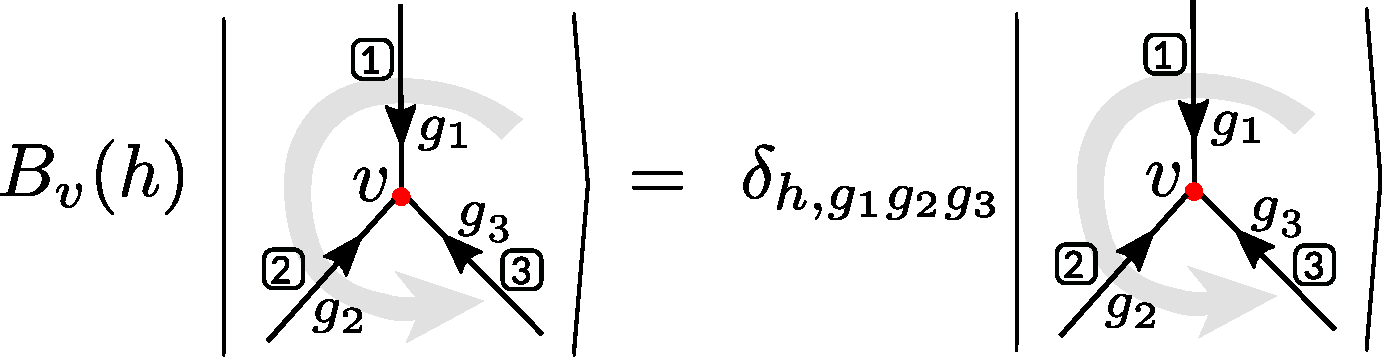
\includegraphics[width= \linewidth]{Figures/B_ops.pdf}
        \caption{Vertex operator. Ordering of the edges is required to make the group multiplication unambiguous. \caro{in addition to the vertex being oriented}}
        \label{eqn:Bs_def}
    \end{subfigure}\hfill
    \begin{subfigure}[b]{0.45\textwidth}
        \centering
        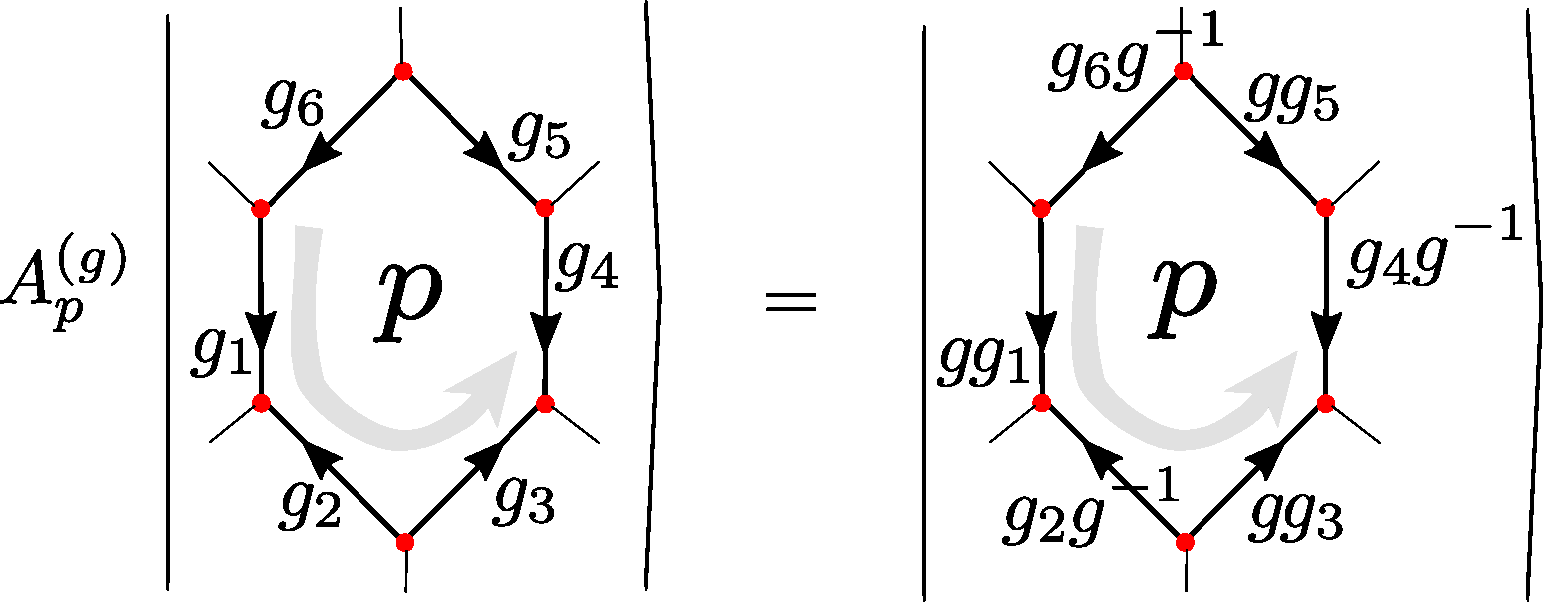
\includegraphics[width = \linewidth]{Figures/A_ops.pdf}
        \caption{Plaquette operator. The orientation of the plaquettes determines pre or post multiplication with the inverse.}
        \label{eqn:As_def}
    \end{subfigure}\hfill
    \caption{The vertex and plaquette operators. \caro{todo: figure does not need a,b, and global caption}}
    \label{fig:vertex_ops}
\end{figure*}



\textbf{Ground State.} The vertex term is diagonal in the basis we defined above, while the plaquette terms are off-diagonal.
However, all terms commute, hence we can diagonalize the Hamiltonian term-by-term and the leftover degeneracy depends only on the genus of the surface our graph is embedded in\cite{Kitaev_2003, cui2018topological}.

% Used to be a Subsection "Ground State"

%The form of the ground state depends heavily on the geometry of the graph the theory is defined on.
%As an example, ground state degeneracy depends on the topology of the manifold the graph is embedded in.

All terms in the Hamiltonian are also projectors, hence, one way to construct a ground state, $\ket{\psi}$, is to apply all the projectors onto a state that has some overlap with the ground state. In particular, we can take the state $\ket{\{e\}}$, where every edge is labelled by the identity element.
This state trivially obeys all $B$-term projectors, so we just need to apply all $A$-term projectors
\begin{equation}
    \ket{\psi} = \prod_{p \in P} \mathbf A_p \ket{\{e\}}.
\end{equation}
The action of the $A$-terms guarantees survival of $\ket{e}$. If the embedding manifold is a 2-sphere, this is the unique ground state and corresponds to the equal weight superposition of all states whose labels respect Gauss' law at each vertex.


% Used to be a Subsection "Excitatons"


%\caro{Move this to GS section}: I do not agree that's better


\textbf{Excitations.} The ground state is stabilized\footnote{Meaning, it is the $+1$ eigenstate.} by the projectors in Eq.~\eqref{eqn:ham}. Together with the property $A_p^{(g_1)}A_p^{(g_2)} = A_p^{(g_1 g_2)}$ this furthermore implies the stronger condition
\begin{equation}
\begin{split}
    A^{(g)}_p \ket{\psi} = \ket{\psi},\\
    B^{(e)}_v \ket{\psi} = \ket{\psi},
\end{split}\label{eqn:ground_state}
\end{equation}
for all $v \in V$, $p \in P$ and $g \in G$. Therefore, the elementary excitation above the ground state will violate one or more of the equations above.

To get a better understanding of the latter, we look at the algebra spanned by the vertex and plaquette operators $B_v$ and $A_p$. But first, we need to put vertices and plaquettes on an equal footing. This is done by pairing plaquettes and adjacent vertices one-to-one into \emph{sites}\footnote{\caro{Of course either some vertices or some plaquettes will be left over depending on the exact geometry of the lattice.}} $s_i = (v_i, p_i)$ such that $A_{s_i}^{(g)} = A_{p_i}^{(g)}$ and $B_{s_i}^{(h)} = B_{v_i}^{(h)}$. 

Operators on different sites commute trivially, while on the same site we have 
\begin{equation}
    \begin{split}
        A_s^{(g)}A_s^{(h)} = A_s^{(gh)}, \\
        B_s^{(g)}B_s^{(h)} = \delta_{g,h} B_s^{(h)},\\
        A_s^{(g)}B_s^{(h)} = B_s^{(ghg^{-1})}A_s^{(g)}.
    \end{split}\label{eqn:alg}
\end{equation}

This is the on-site representation of the quantum double algebra of a finite group $G$, $D(G)$. The algebraic relations in Eq.~\eqref{eqn:alg} do not depend on the exact grouping of plaquettes and vertices into sites.

The on-site excitations are labelled by the irreducible representations of this algebra \cite{cui2018topological, Kitaev_2003}. In particular, the ground state is the state with the trivial (charge free) representation on each site. 
%\caro{At some point we need to introduce the notion of pure charge, pure flux and a dyon, we should state the simplified expressions for pure charge and pure flux, and the notion of generalized conjugation in the dyon case, as we use this later on.}

The irreducible representations of this algebra are labelled by two objects, a conjugacy class $C$ of the group $G$ and an irreducible representation $\chi$ of the centralizer of the class representative $Z(r)$, with $r \in C$. The vector space on which $(C, \chi)$ acts is spanned by a basis $\ket{\mu} = \ket{c, i}$, where $c \in C$ and $i \in \{1, 2, \ldots, \text{dim}\chi\}$, i.e. the first index goes over the conjugacy class elements while the second goes over the vector indices of the irreducible representation $\chi$.


The action of the algebra generators on this vector space is
\caro{what happens with $i,i'$ in the first line?} 
\begin{equation}
    \begin{split}
        B^{(h)}_{\mu\nu}=\bra{c, i} B^{(h)} \ket{c', i'} = \delta_{c, h} \delta_{c, c'}, \\
        A^{(g)}_{\mu\nu} = \bra{c, i} A^{(g)} \ket{c', i'} = \delta_{c,gc'g^{-1}} \Gamma^\chi_{ii'}(q_{c}^{-1}gq_{c'}),
    \end{split}
\end{equation}
where $\Gamma$ is the $\chi$-representation matrix and $q_c$ is a group element that satisfies $q_c c q_c^{-1} = r$. Note that $q_c^{-1}gq_{c'} \in Z(r)$ for all $g$ such that $c = gc'g^{-1}$ and that the $B$-matrices do not depend on the second label in $\ket{c, i}$.
%\caro{omit: These representation matrices are going to play a central role in our protocols for creating and manipulating anyons.}

As an example, the aforementioned vacuum (or trivial) representation, labelled by $(\{e\}, \mathbb{1})$, is one-dimensional and spanned by $\ket{e, 0}$:
\begin{equation}
    \begin{split}
        B^{(h)}\ket{e, 0} = \delta_{h,e}\ket{e, 0},\\
        A^{(g)}\ket{e, 0} = \ket{e,0},
    \end{split}
\end{equation}
hence Eq.~\eqref{eqn:ground_state} implies that the ground state is such that every site houses a trivial representation.

Other important examples are pure charges and fluxes. A pure flux is labelled by a conjugacy class and the trivial representation of its centre, $(C, \mathbb{1})$. Its basis vectors are $\ket{c, 0}$ for $c \in C$, with
\begin{equation}
    \begin{split}
        B^{(h)}_{\mu\nu}=\bra{c, 0} B^{(h)} \ket{c', 0} = \delta_{c, h} \delta_{c, c'}, \\
        A^{(g)}_{\mu\nu} = \bra{c, 0} A^{(g)} \ket{c', 0} = \delta_{c,gc'g^{-1}}.
    \end{split}
\end{equation}
Pure flux excitations only violate the the vertex term.

Pure charge excitations are labelled by the group identity and a representation of the group $G$ itself, $(\{e\}, \chi)$. Its basis vectors are $\ket{e, i}$ for $i \in \{1, 2, \ldots, \text{dim}\chi\}$, with
\begin{equation}
    \begin{split}
        B^{(h)}_{\mu\nu}=\bra{e, i} B^{(h)} \ket{e, i'} = \delta_{e, h},\\
        A^{(g)}_{\mu\nu} = \bra{e, i} A^{(g)} \ket{e, i'} = \Gamma^\chi_{ii'}(g).
    \end{split}
\end{equation}
Pure charge excitations only violate the plaquette term.


In particular, if we have a gauge field state, $\ket{\chi, p; i}$, where each site houses a trivial representation except for one, $(v, p)$, which is occupied by a pure charge $(\{e\}, \chi)$, this state satisfies all the constraints in Eq.~\eqref{eqn:ground_state} except for
\begin{equation}
    A_p^{(g)}\ket{\chi, p; i} = \sum_{i'} \Gamma^\chi_{ii'}(g)\ket{\chi, p; i'},\label{eqn:tranfs}
\end{equation}
where $i$ and $i'$ are the internal degrees of freedom of the charge\footnote{Note that the charge can be vector valued for non-abelian symmetry groups.}.
This is the way a charged state transforms under gauge transformations in gauge field theory. Hence, we say that the plaquette terms generate gauge transformations.

All other anyons are called dyons. They violate vertex and plaquette terms simultaneously, meaning they have a flux component associated with a vertex of the site $(v,p)$ and a charge component associated with its plaquette. In nonabelian theories, the two components are not separable.


\subsection{Ribbon Operators}

In the following, we will explain how to create and manipulate the excitations we have classified above.

The excitations are always created in pairs from the vacuum. To see why, imagine we take the ground state and shift the label of one of the legs, $e_0 \in E$, by $G$-multiplying it by some constant group element, i.e. $f(e_0) \rightarrow gf(e_0)$ for all labellings $f: E \rightarrow G$ in the superposition, this action disturbs two vertex operators $B^{(e)}_{e_0^+}$ and $B^{(e)}_{e_0^-}$ on each end of the leg $e_0$.

There exists a set of such line/ribbon operators that when acted upon a ground state create two excitations on both of its ends. These operators are labelled by the elementary excitations they create, $(C, \chi)$.

If the ribbons are closed, they leave the ground state unchanged, since there are no ends. Moreover, they span all (loop) operators that leave the ground state invariant, it is in that way that the quantum double ground state knows about the quasiparticle spectrum.

The ribbon operators are constructed in Ref \cite{}. These operators represent a planar diagram algebra generated by the specific Braiding Tensor Category (BTC) and hence were conceived as a model that can perform fault-tolerant quantum computing by the means of braiding anyons. 

However, even though the braid group itself is universal \cite{} its image on this planar diagram algebra is finite, hence non-universal. For some gauge groups it can be made universal by the addition of measurements, but it will not be the case for our example.

The ribbon operators are not unitary in general. If the anyons have an internal dimension larger than one, the operators that create and manipulate the excitations are non-local projectors (or unitarily related to projectors). This is a problem when compiling unitary quantum circuits for braiding anyons. In Ref. \cite{} the group overcame this issue by the means of unitary lattice deformations, rotating from a state with a set of nonabelian anyons on one graph to another state with the same anyon content but defined on another graph, hence they were able to move the internal dimension-1/2 (majorana fermions) anyons unitarily. However, these are extrinsic and static lattice defects on top of a theory that is an Abelian $\mathbb Z_2$ gauge theory, hence, the nature of theirs and our nonabelian anyons is different.

\subsubsection{Application Scheme}
We are going to describe a scheme by which we implement these non-local projecting ribbon operators.

It starts by identifying the anyon type and the representation associated with them. 

Say we have a ribbon of type $(C, \chi)$ of dimension $d = \text{dim}(C, \chi)$. There are a couple of interpretations of the dimension $d$, one is that the anyons carry an internal spin-like degree of freedom encoded in the gauge field itself, another one is that the fusion outcomes span a $d\times d$ space of the representation $(C, \chi) \otimes (C, \chi)$, individual outcomes being the subspaces in the Clebsch-Gordan decomposition.

Note that the fusion outcome is a non-local degree of freedom once the anyons are separated, this being the main idea of fault-tolerant topological quantum computing.

We, however, require storing this information locally since we need to do measurements on this space as we move the anyons. This is done by keeping one auxiliary qudit per anyon/end of the ribbon.

Every ribbon is made up from two main kinds of elementary triangles, see Figure \ref{}. If we imagine that appending elementary triangles onto a ribbon is moving the anyons at the ribbon's end by elongating the ribbon, the two kinds are: \begin{itemize}
    \item Type I) Triangles whose side follows the leg it touches, whose edges include two vertices and one plaquette. These triangles move the flux component of the anyon from the first vertex to the second vertex.
    \item Type II) Triangles which cross the leg it touches, whose edges include two plaquettes and one vertex. these triangles move the charge component of the anyon from the first plaquette to the second plaquette.
\end{itemize}

The type of the triangle determines the step \textbf{2.} of the algorithm we are about to describe. This step will also depend on the exact configuration of leg orientation, ribbon orientation etc., see Figure \ref{} and Appendix \ref{app:ribs} for an exhaustive list.


\todo{Figure Ribbon Example: An example of a ribbon decomposed into elementary triangles}

\todo{Figure Triangles: Figure showing the 16 types of triangles: [(I, II), (R, L), (in, out), (f, b)]}

%\caro{You do that sequentially, i.e., not just 'for all $t_i$' but one after another. Also, would be easier to just talk about a forward moving ribbon where you only have $|c,i\rangle$ and $|g\rangle$ and then consider backwards in an appendix} I would still include both qubits, since there are two indices in the def. of F

\textbf{The algorithm} that creates two anyons along a ribbon path $R$ made up from a set of triangles $R = \{t_1, t_2, \ldots, t_N\}$ in the internal state: $\ket{\alpha; \beta} = \ket{c', i'; c, i}$ i.e. applying $F_{\alpha, \beta}^{(C,\chi)}(R)$ is:\begin{enumerate}
    \item Initialize the two auxiliary qudits in the states $\ket{\alpha, \beta}$. We will think of the first qudit as the ribbon's backend and the second as its frontend.
    \item Focusing on one case of many: growing the ribbon from $t_1$ onwards, for each $t_i$ sequentially in R do one of the following unitaries depending on the type and orientation of the triangle: \begin{enumerate}
        \item Type I) Multiply the label of the $t_i$'s leg by the group element encoded by the forward auxiliary qudit: $\ket{c', i';c, i}\ket{g}_{t_i} \rightarrow \ket{c', i';c, i}\ket{cg}_{t_i}$.
        \item Type II) (Generalize-)Conjugate the forward axially qudit by the label of the leg crossed by $t_i$: $\ket{\alpha;\beta}\ket{g}_{t_i} \rightarrow \sum_\gamma A_{\gamma\beta}^{(g)}\ket{\alpha;\gamma}\ket{g}_{t_i}$.
    \end{enumerate}
    \item Project the ancillary qudits to a Bell-pair state: $\bra{\Phi^+} = \frac{1}{\sqrt{d}}\sum_\nu \bra{\nu; \nu}$.
\end{enumerate}

This procedure creates a pair of excitations on the ends of a ribbon $R$ of type $(C, \chi)$ in an internal (fusion) state $\ket{\alpha, \beta}$. \jovan{Needs better wording.}

The matrices $A^{(g)}$ are the representation matrices for the irreducible representation $(C, \chi)$. The projection is done by measurement and post-selection (or error correction).

For the other variants of Step \textbf{2.}, for different leg orientations etc., consult the Appendix \ref{app:ribs} and Figure \ref{}. 

In the way presented above, we have started building up the ribbon from start-to-finish using only forward-type elementary triangles. Similarly, we could have started in the middle and extend in parallel both forward and backwards with appropriate types of elementary triangles, see Appendix \ref{app:ribs}. Backwards-type elementary triangles, analogously to Step \textbf{2.} stated above, act with the backwards auxiliary qudit.

As we can see the operation is sequential so at best the depth of a circuit implementing this is $\mathcal{O}(|R|)$, with the best depth achieved by starting at the middle and growing it both ways.

Of course, we can make this constant depth by separating the main Ribbon into $|R|$ smaller ribbons which however requires $|R|$ pairs of qudits and Bell-pair measurements, needing an exponential  in $|R|$ number of repetitions for a $\mathcal{O}(1)$ number of successful applications.

To interpret what we have here, let us look at the quantum recourses. We have the qudits representing the matter $\mathcal{H}_{\text{matter}}$ and the ancillary bits representing the internal state of the anyons, or the fusion space, $\mathcal{H}_{\text{ancilas}} \equiv \mathcal{H}_{\text{fusion}}$ which is already embedded non-locally in  $\mathcal{H}_{\text{matter}}$.

The two types of triangles couple the two spaces in two different ways, for Type I the $\mathcal{H}_{\text{ancilas}}$ controls an action on $\mathcal{H}_{\text{matter}}$ and for Type II it is the other way around. After the measurement that disentangles, the redundant copy of $\mathcal{H}_{\text{fusion}}$ the $\mathcal{H}_{\text{matter}}$ is left in a state with the ribbon operator imprinted on it as signalled by the topological charge, braiding amplitude and phase.

\subsection{Reduced Charge Measurement}
%\caro{Explain the idea of reduced charge measurement in words, i.e., get partial information and combine the partial information for different $H$ to deduce charge}

In this section, we will explain how we measure charge, the last element of our toolkit for probing topological order. The main idea of our protocol is to construct weak topological charge measurements that are easy to implement in terms of circuit depth. However, such weak measurements do not determine the charge completely, but when we combine a set of such weak measurement results we are able to deduce the full charge content of a region of our system.

The ideal charge measurement would differentiate any type of excitation on any site, such measurement is associated with the following set of projectors \cite{}:
\begin{equation}
    P_s^{(C, \chi)} = \frac{\chi(e)}{|Z(r)|}\sum_{c \in C}\sum_{z \in Z(r)}\chi^*(z)B_s^{(c)}A_s^{(q_c z \bar{q}_c)},
\end{equation}
for each irreducible representation of the $D(G)$.

Since we work in a basis where projectors onto a given $G$-valued flux through a vertex $v$, $B_v^{(h)}$, are diagonal, we can just do a full projective measurement of our gauge field degrees of freedom in that basis. 
The result of such measurement is a labelling, $f: E \rightarrow G$ from which we just compute the flux through any vertex. 

However, the problem lies in measuring the (off-diagonal) charge component of the full topological charge.
This problem is implementing a controlled $A^{(g)}_s$ operator which needs a controlled group multiplication applied to all legs of $s$'s plaquette, i.e. $\ket{g}\ket{g_i} \rightarrow \ket{g}\ket{gg_i}$ for all $\ket{g_i}$ around the plaquette.
This, in the case of non-abelian groups, such as $D_4$, is prohibitively expensive. 

% Used to be a subsection: {Reduced Charge Measurement}

%\caro{general comment: just talk about the reduced charge measurement, make the purpose of it clear in the first few sentences: reduced circuit depth is traded for only gaining partial information because measurement outcomes for a single subgroup are compatible with several charges, repeating the measurement for different subgroups allows to deduce charge uniquely for examples considered (D4, Q8), skip all of the following until}

The key idea behind the weak measurement protocol is that controlled $A_s^{(g)}$ becomes significantly simpler to perform once we restrict ourselves to a proper subset of the full group, i.e. $g \in H \subset G$.
This restriction is the key to greatly reduce the complexity of the circuit, in terms of depth, for measuring the topological charge,
%\caro{the figure here is too early and does make little sense, we need to introduce the encoding first, we also need to explain why toffoli are so costly, bc here it looks like depth 6 to depth 3}
see Section \ref{subsec:enc} for full details.

With Eq.~\eqref{eqn:tranfs} in mind, we propose the following protocol:

\textbf{The algorithm} for the $H$-reduced charge measurement on a plaquette $p$:\begin{enumerate}
    \item Prepare an auxiliary qudit, $a$, encoding the elements of $H\subset G$, in an equal superposition over all elements, so that the joint total state of the system is: $$ \sum_{h \in H} \ket{h}_a\ket{\psi}_{G.F.}. $$
    \item Apply a $a$-controlled $G$-multiplication unitary onto the legs touching the plaquette $p$:$$ \sum_{h \in H} \ket{h}_a\ket{\psi}_{G.F.} \rightarrow \sum_{h \in H} \ket{h}_a A^{(h)}_p \ket{\psi}_{G.F.}. $$
    \item Apply a unitary $$ U_a = \sum_{\chi_H}\sum_{i', j'}\sum_{h'\in H}  \Gamma^{\chi_H}_{i'j'}(h')  \ket{\chi_H; i', j'}_a\bra{h'}_a $$ onto the auxiliary qudit $a$. Here the $\chi_H$ labels the irreducible representations of $H \subset G$, $\Gamma^{\chi_H}(h')$ are the representation matrices, with $i'$ and $j'$ being the vector indices for a given representation $\chi_H$.
    \item Measure the auxiliary qudit $a$.
\end{enumerate}

%Needs a case example
To see how this protocol works, let us examine a following case.
Take the gauge field in a state of well-defined pure charge on a plaquette $p$: $\ket{\psi}_{G.F.} = \ket{\chi, p; i}$.

Using the Eq.~\eqref{eqn:tranfs} we can write the joint state after Step \textbf{2.} as:
\begin{equation}
    \sum_{h \in H} \ket{h}_a A^{(h)}_p \ket{\chi, p; i} = \sum_{h \in H} \ket{h}_a \Gamma^{\chi}_{ij}(h) \ket{\chi, p; j}.
\end{equation}

Let us also take $H = G$, in which case this becomes a full charge measurement. The unitary $U_a$ is then: \begin{equation}
    U_a = \sum_{\chi'}\sum_{i', j'}\sum_{h'\in G}  \Gamma^{\chi'}_{i'j'}(h') \ket{\chi'; i', j'}_a\bra{h'}_a.
\end{equation}

The joint state after Step \textbf{3.} becomes:\begin{equation}
    \begin{split}
        \sum_{h \in G} U_a\ket{h}_a \Gamma^{\chi}_{ij}(h) \ket{\chi, p; j} = \\
        \sum_{h \in G} \sum_{\chi'}\sum_{i', j'}  \Gamma^{\chi'}_{i'j'}(h)\Gamma^{\chi}_{ij}(h) \ket{\chi'; i', j'}_a \ket{\chi, p; j} =\\
        \sum_j\ket{\chi; i, j}_a \ket{\chi, p; j}
    \end{split}
\end{equation}

The decoupling we see in the last line after summing over $h$ is guaranteed by the Schur's orthogonality lemma, the orthogonality lemma is the main reason for suggesting the form of the decoupling unitary $U_a$ we have suggested.

In the case above, the result of the measurement in Step \textbf{4.} is a label $(\chi, i, j)$, representing the charge, the internal state before the measurement and the internal state after the measurement.

If we, however, take $H \subset G$, then the charge information is partial.
By partial charge information, we mean that the result of the measurement protocol, the label $(\chi_H, i, j)$ is no longer compatible with only one charge but a set of charges, i.e. charge is not fully determined.

We may repeat the procedure using different subgroups of $G$ to gather further partial information on the charge in the hope that we may be able to deduce the charge fully. \jovan{Needs better wording.}

This relies on partial orthogonality of character tables of a group and its subgroup, and is best explored in the specific cases below.

\subsubsection{Specific example of $D_4$}

In this section, we explore the reduced charge measurement in the case of $D_4$ gauge group.
Limiting ourselves to only pure charges, remembering that the flux component can be directly read out, we have five possibilities for topological charge on a site: $0$, $\Sigma_r$, $\Sigma_m$, $\Sigma_{mr}$ and $\Sigma_{\epsilon}$. Please consult the Appendix \ref{app:reps} for the list of all representations of $D(D_4)$.

The traces of the representation matrices $\sum_i\Gamma^\chi_{ii}(g) = \chi(g)$ for the five flavours are given in Table \ref{tab:char}. This is the character table of $D_4$ and the association between the irreps and topological charges mentioned above are: $1 \rightarrow 0$, $\alpha_x \rightarrow \Sigma_x$ and $\epsilon \rightarrow \Sigma_\epsilon$.

\begin{table}[h]
\centering    \begin{tabular}{c|c c c c c }
         %\hline
         $D_4$ & $\mathcal C_e$ & $\mathcal C_{r^2}$ & $\mathcal C_{r}$ & $\mathcal C_m$ & $\mathcal C_{mr}$ \\
         \hline
         $1$ & 1 & 1 & 1 & 1 & 1 \\
        % \hline
         $\alpha_r $& 1 & 1 & 1 & -1 & -1  \\
         %\hline
         $\alpha_{m}$ & 1 & 1 & -1 & 1 & -1  \\
         %\hline
         $\alpha_{mr}$ & 1 & 1 & -1 & -1 & 1  \\
         %\hline
         $\epsilon$ & 2 & -2 & 0 & 0 & 0  \\
         %\hline 
    \end{tabular}
    \caption{Character table of $D_4$.}\label{tab:char}
\end{table}

All the proper subgroups of $D_4$ are abelian, hence all the $\chi_H$ are one dimensional, this means that the measurement outcome of the reduced charge measurement is just the irrep label $(\chi_H)$.

We will focus on the three four element subgroups $H_r = \{e, r, r^2, r^3\} \equiv \mathbb{Z}_4$, $H_m = \{e, r^2, mr^2, mr^2\} \equiv \mathbb{Z}_2 \times \mathbb{Z}_2$ and $H_{mr} = \{e, r^2, mr, mr^3\} \equiv \mathbb{Z}_2 \times \mathbb{Z}_2$.

The partial orthogonality of irreps of $D_4$ and these three groups is captured in the quantity: $ \braket{\chi, \chi_H} = \sum_h \chi(h)\chi_H(h)$. This is shown in Table \ref{tab:red_ch}, see the Appendix \ref{app:reps} for the list of irreps of subgroups of $D_4$.


\begin{table}[h]
\centering
\begin{tabular}{l|lllll}
  $\braket{\chi_{H_m}, \chi}$ & $1$ & $\alpha_{r}$ & $\alpha_{m}$ & $\alpha_{mr}$ & $\alpha_{\epsilon}$ \\ \hline
$(1,1)$ & 4   & 0            & 4             & 0               & 0                   \\ 
$ (1,-1)$ & 0   & 4            & 0             & 4               & 0                   \\ 
$(-1,1)$ & 0   & 0            & 0             & 0               & 4                   \\ 
$(-1,-1)$ & 0   & 0            & 0             & 0               & 4                   \\ 
\end{tabular}
\begin{tabular}{l|lllll}
  $\braket{\chi_{H_{mr}}, \chi}$ & $1$ & $\alpha_{r}$ & $\alpha_{m}$ & $\alpha_{mr}$ & $\alpha_{\epsilon}$ \\ \hline
$(1,1)$ & 4   & 0            & 0             & 4               & 0                   \\ 
$ (1,-1)$ & 0   & 4            & 4             & 0               & 0                   \\ 
$(-1,1)$ & 0   & 0            & 0             & 0               & 4                   \\ 
$(-1,-1)$ & 0   & 0            & 0             & 0               & 4                   \\ 
\end{tabular}
\begin{tabular}{l|lllll}
  $\braket{\chi_{H_r}, \chi}$ & $1$ & $\alpha_{r}$ & $\alpha_{m}$ & $\alpha_{mr}$ & $\alpha_{\epsilon}$ \\ \hline
$1$ & 4   & 4            & 0             & 0               & 0                   \\ 
$-1$ & 0   & 0            & 4             & 4               & 0                   \\ 
$i$ & 0   & 0            & 0             & 0               & 4                   \\ 
$-i$ & 0   & 0            & 0             & 0               & 4                   \\ 
\end{tabular}
\caption{Partial orthogonality of $D_4$ with respect to its three four-element subgroups.}
\label{tab:red_ch}
\end{table}

%\caro{What about the $\pm i$ outcomes for $H_r$? we can't measure $\pm i$.} See encoding.

The Table \ref{tab:red_ch} is to be interpreted as follows, imagine we performed a $H_m$-reduced charge measurement on a plaquette $p$ and got a label $(1,1)$. This label has a non-vanishing overlap with $1$ and $\alpha_m$, hence both $0$ and $\Sigma_m$ can be on a plaquette $p$.

Now imagine we have performed all three measurement and got a set of labels $\{(1, 1), (1, -1), -1\}$, this set is only compatible with $\alpha_m$ and hence $\Sigma_m$ must be on a plaquette $p$.

%\caro{We are more interested in the inverse direction, namely, the result $\{(1,-1); (1,-1); 1\}$ is only compatible with charge $\Sigma_r$.} Agreed, better phrasing.

The main advantage of doing these three measurements instead of a full charge measurement is twofold, both the controlled multiply unitary $U_{\text{CM}}: \ket{h, g} \rightarrow \ket{h, hg}$ and the decoupling unitary $U_a$ are much simpler if we restrict ourselves to $h \in H \subset G$.


\section{Braiding Experiments and Numerical Results}

In this chapter, we will present a set of braiding protocols that fully demonstrate the braiding statistics of the $D_4$ lattice gauge theory excitations. These also generate all the braiding amplitudes of the braiding protocols, however direct evaluation of longer protocols on current NISQ hardware is prohibited by the limitation on the circuit depth imposed by the noise, as the reader will see in the next chapter. 

The main experiments showcasing the nonabelian nature of the excitations are as follows:

i) anyon fusion; the fusion outcome doesn't have an unique topological charge,

ii) nonabelian braiding; the braiding amplitude changes as we change the order of braids,

iii) \caro{full S- and T-matrix measurement; this generates the complete UTC data that specifies any braiding amplitude.
%Technically speaking, the UMTC data is not captured by S and T matrix alone
} 
 
It is easy to obtain the results of the first two experiments from the result of the last one, however it is useful to consider the two foundational phenomenological facts pertaining to the nonabelian anyons in separate points.

\subsection{Encoding, Ribbon operators and Charge Measurements}\label{subsec:enc}

In this section, we will discuss the $D_4$ group element encoding and group operation circuits based around this encoding.

\textbf{The Encoding.} The states of the gauge field are characterized by group element labelings of the legs of the graph.
In general, our degrees of freedom are group valued.
The cardinality of $D_4$ is 8, hence we need three qubits to encode a group element.
We chose the following map
\begin{equation}
    \ket{g} \equiv \ket{a}_m\ket{b}_r\ket{c}_{r^2} \iff g = m^a r^b (r^2)^c,
\end{equation}
where $a,b,c \in \{0,1\}$ and $r$ is the $90^{\text{o}}$ rotations and $m$ is the reflection.

When encoding the internal space of the anyon, which we need for our ribbon operator protocol, we note that the basis also include a group element component: $\ket{\nu} = \ket{c, i}$, where $c \in C_x$, for some conjugacy class.
The elements of a conjugacy class are also encoded similarly, for example, $C_r = \{r, r^3\}$:
\begin{equation}
    \ket{c} \equiv \ket{a}_{r^2} \iff c = m^0r^1(r^2)^a,
\end{equation}
using only one qubit.

This also hold for encoding elements of a subgroup:
\begin{equation}
    \ket{h} \equiv \ket{a}_r\ket{b}_{r^2} \iff h = m^0r^a(r^2)^b,
\end{equation}
for the example of $h \in H_r$.

%These \caro{restrictions%these are not really restrictions, maybe say that we often just need to multiply with elements from a certain conjugacy class as indicated by the ribbon operator prescriptions in Eq. sth and that for this purpose we can use a single qubit and a circuit that is much shorter than the general group multiplication circuit.
%} 
%not only reduce the number of bits needed, but also greatly reduce the complexity of circuits implementing %various group operations.

The restriction of the domain of the controlled $G$-multiplication unitary map not only reduce the number of qubits needed to encode the inputs, but also greatly reduce the depth of the circuit implementing the map, which we will see very shortly.

However, before talking about the circuits, we would lastly note that there is no natural way to encode the representations of the subgroups $\chi_H$, hence for $H_m$ and $H_{mr}$ we will use:
\begin{equation}
    \ket{(-1)^a,(-1)^b} \equiv \ket{a,b},
\end{equation}
while:
\begin{equation}
    \ket{i^{2a+b}} \equiv \ket{a, b}.
\end{equation}

%\caro{
%Let us return to circuits implementing group operation. We already presented some in Figure \ref{fig:restMult} in order to showcase the great simplifications of group multiplication when someone restricts the domain of the multiplication unitary, $U_{\text{CM}}: \ket{g, h} \rightarrow \ket{g, gh}$, from the full group to a subgroup and a single conjugacy class.
%This is the first time we actually discuss circuits. How about we start off with 'we need group multiplication and conjugation', these are the general circuits that do these two operations, they are long bc they involve x number of tofollis. however for ribbons we need only group multiplication for elements of conjugacy class which reduces circuit depths significantly, then include fig:restMult
%}

\textbf{The Circuits.} For the rest of the section, we will focus on circuits implementing the group related operations appearing in our protocols. These operations include:\begin{itemize}
    \item Controlled $G$-multiplication, $U_{\text{CM}}: \ket{g, h} \rightarrow \ket{g, gh}$, of both full and restricted domain of the input:\begin{enumerate}
        \item full domain variant ($g \in G$) is used for ground state preparation, see the next section.
        \item domain restricted to a conjugacy class variant ($g \in C$) is used in ribbon operator application protocol.
        \item domain restricted to a four element subgroup variant ($g \in H$) is used in $H$-reduced charge measurement. 
    \end{enumerate}
    \item Controlled generalized $(C, \chi)$-conjugation, $U_{\text{GC}}: \ket{\alpha}\ket{g} \rightarrow (A^{(g)}\ket{\alpha}\ket{g})$, with $A^{(g)}$ being the representation matrices of the $(C, \chi)$ representation, used in ribbon operator application protocol.
    \item The decoupling unitary of the $H$-reduced charge measurement: $$ U_a = \sum_{\chi_H}\sum_{i', j'}\sum_{h'\in H}  \Gamma^{\chi_H}_{i'j'}(h')  \ket{\chi_H; i', j'}_a\bra{h'}_a. $$
\end{itemize} 

The full list of circuits for all variants of the above-mentioned operations are presented in Appendix \ref{app:cirqs}.
We will now focus on a set of examples illustrating the expected circuit depths.

A sample of controlled multiply circuits, both of full and restricted domain, are shown in Figure \ref{fig:restMult}. We must note that a 3-qubit Toffoli gate must be compiled in terms of 2-qubit coupling gates, which is true for almost all quantum simulators, since they cannot perform Toffoli gates natively. Hence, each Toffoli gate should be seen as a depth-6 circuit in itself. With this in mind, we can appreciate a dramatic reduction of circuit depth achieved by restricting the domain of the controlled multiplication circuit.

This is one of the main facts that allows us to greatly simplify many circuits related to ribbon operators and reduced charge measurement. However, the direct ground state preparation doesn't benefit from these simplifications.

We saw that the ribbon operators are made up from two types of elementary triangles. The first require group multiplication maps, restricted to a single conjugacy class, from the auxiliary degree of freedom onto the matter. The other are acting the other way around, implementing a specific representation of the group transformation onto the auxiliary degree of freedom controlled by the matter, a controlled generalized $(C, \chi)$-conjugation map.

Let us look at the circuits involved in the ribbon application protocol for two different anyon flavours, a pure $m$-flux $\Psi_m \equiv (C_m, (1,1))$ and a $m$-dyon $\tilde{\Phi}_m \equiv (C_m, (-1, -1))$. These two anyons differ notably in how difficult it is to create and manipulate them, as we will see. The representation matrices $A^{(g)}$ for the two representations are shown in Figure \ref{tab:somereps}. The full list of the representations is discussed in Appendix \ref{app:reps}.

\begin{table}[]
    \centering
    \begin{tabular}{|p{0.5cm}||p{0.25cm}|p{0.5cm}|p{0.5cm}|p{0.6cm}|p{0.5cm}|p{0.5cm}|p{0.5cm}|p{0.5cm}|}
    \hline
  $A^{(g)}$ & $e$ &   $r$ & $r^2$ & $r^3$ &  $m$ & $mr$ & $mr^2$ & $mr^3$ \\
\hline\hline
 $\Psi_{m}$ &$\mathbb{1}$&  $\sigma_x$ & $\mathbb{1}$&  $\sigma_x$ & $\mathbb{1}$& $\sigma_x$ &  $\mathbb{1}$&   $\sigma_x$ \\\hline
 $\tilde{\Phi}_{m}$ &$\mathbb{1}$&$i\sigma_y$ &$-\mathbb{1}$& $-i\sigma_y$ &$-\sigma_z$ &$-\sigma_x$ &  $\sigma_z$ &   $\sigma_x$ \\\hline
\end{tabular}
    \caption{$A^{(g)}$ matrices for $\Psi_m$ and $\tilde{\Phi}_m$ representation of $D(D_4)$.}
    \label{tab:somereps}
\end{table}

These two representations are two-dimensional, anyons are non-abelian and have an internal state space spanned by vectors: $\{\ket{m; ++}, \ket{mr^2; ++}\}$ for $\Psi_m$ and $\{\ket{m; --}, \ket{mr^2; --}\}$ for $\tilde{\Phi}_m$.
This space is encodable with a single auxiliary qubit for each anyon, $\ket{a}_{\text{aux}} \equiv \ket{m(r^2)^a; \sigma\sigma}$.

The matter will act on this space every time an anyon crosses some leg $i$ via $U_{\text{GC}}: \ket{a}\ket{g}_i \rightarrow (A^{(g)}\ket{a})\ket{g}_i$, which we need to compile.
The circuits for this operation are shown in Figure \ref{fig:genConj} (Left and Center).
It is easy to check that these circuits agree with the representation matrices given in Table \ref{tab:somereps}. 
The auxiliary space acts on the matter every time an anyon moves along a leg $i$ via $U_{\text{CM}}: \ket{a}\ket{g}_i \rightarrow \ket{a}\ket{m(r^2)^a g}_i$, the circuit which performs this operation is shown in Figure \ref{fig:genConj} (Right).

\begin{figure}
\begin{equation*}
\Qcircuit @C=0.4em @R=0.7em @!R{
\lstick{m} & \qw & \ctrl{3} & \qw & \qw & \qw & \qw\\
\lstick{R} & \ctrl{2} & \qw & \ctrl{3} & \ctrl{3} & \qw & \qw\\
\lstick{R^{2}} & \qw  & \qw & \qw & \qw & \ctrl{3} & \qw
\\
\lstick{\quad m} &  \ctrl{2} & \targ & \qw & \qw & \qw & \qw\\
\lstick{R} & \qw & \qw & \ctrl{1} & \targ & \qw & \qw\\
\lstick{R^{2}} & \targ & \qw & \targ & \qw & \targ & \qw
}\qquad\qquad
\Qcircuit @C=0.4em @R=0.7em @!R{
\lstick{mR} & \ctrl{2} & \ctrl{3} & \qw & \qw\\
\lstick{R^{2}} & \qw  & \qw & \ctrl{3} & \qw
\\
\lstick{\quad m} &  \targ & \qw & \qw & \qw \\
\lstick{R} & \qw & \targ & \qw & \qw\\
\lstick{R^{2}} & \qw & \qw & \targ & \qw
}\qquad\qquad
\Qcircuit @C=0.4em @R=0.7em @!R{
\lstick{R^{2}} & \qw  & \ctrl{3} & \qw
\\
\lstick{\quad m} &  \gate{X} & \qw & \qw \\
\lstick{R} & \qw & \qw & \qw\\
\lstick{R^{2}} & \qw & \targ & \qw
}
\end{equation*}

    \caption{Group multiplication circuits: $U_{\text{CM}}:\ket{g,h} \rightarrow \ket{g,gh}$. Left: Both $g$ and $h$ are unrestricted to be any element of the group $G$, the first three qubits encode the first elements and the second three the second element. Center: The first element is restricted to be in $H_{mr}$ subgroup and is encoded by just the first two qubits. Left: The first element is restricted to be in $C_m$ conjugacy class and is encoded by just the first qubit. Given that the 3-qubit Toffoli gate needs to be compiled into a depth-6 circuit involving 2-qubit gates to be implementable, notice the dramatic decrease in depth when the inputs are restricted to a subset of the full group.}
    \label{fig:restMult}
\end{figure}

\begin{figure}
\begin{equation*}
\begin{split}
\Qcircuit @C=0.5em @R=0.7em @!R{
\lstick{m} & \qw & \qw \\
\lstick{R} & \ctrl{2}  & \qw \\
\lstick{R^{2}} & \qw  & \qw \\
\lstick{\text{aux}} &  \targ & \qw
}\qquad\qquad
\Qcircuit @C=0.5em @R=0.7em @!R{
\lstick{m} & \ctrl{3} & \qw & \gate{Z} & \qw\\
\lstick{R} & \qw & \ctrl{2} & \gate{S} & \qw\\
\lstick{R^{2}} & \qw  & \qw & \gate{Z} & \qw\\
\lstick{\text{aux}} & \gate{Z}  & \gate{Y} & \qw & \qw 
}\qquad\qquad
\Qcircuit @C=0.5em @R=0.7em @!R{
\lstick{m} & \gate{X} & \qw \\
\lstick{R} & \qw  & \qw \\
\lstick{R^{2}} & \targ  & \qw \\
\lstick{\text{aux}} &  \ctrl{-1} & \qw
}
\end{split}
\end{equation*}
 
    \caption{Circuits involved in anyon manipulation, ribbon operators. The first three qubits encode the physical, group valued, degree of freedom of the gauge field; the last qubit encodes the auxiliary bit representing the internal state of the (two-dimensional) anyon. Left: the conjugation unitary $U_{\text{C}}: \ket{c; ++}\ket{g}_i \rightarrow \ket{gcg^{-1}; ++}\ket{g}_i$ used when the pure flux $\Psi_m$ crosses a leg $i$. Middle: the generalized conjugation unitary $U_{\text{GC}}: \ket{c: --}\ket{g}_i \rightarrow (A^{(g)}\ket{c; --})\ket{g}_i$ used when a dyon $\tilde{\Phi}_m$ crosses a leg $i$. Right: multiplication unitary $U_{\text{CM}}: \ket{c; \sigma\sigma}\ket{g}_i \rightarrow\ket{c; \sigma\sigma}\ket{cg}$ used when either of the two mentioned anyons moves along a physical leg $i$. Note: $\ket{c; \sigma\sigma} = \ket{a}_{\text{aux}} \iff c = m(r^2)^a$, for $a\in\{0,1\}$. The Pauli-$S$ gate is a phase gate: $S = \text{diag}(1, i)$. \jovan{Neds cleaner wording.}}
    \label{fig:genConj}
\end{figure}

\begin{figure}
\begin{equation*}
\begin{split}
\Qcircuit @C=0.5em @R=0.7em @!R{
\lstick{a} & \gate{H} & \qw \\
\lstick{b} & \gate{H}  & \qw
}\qquad\qquad
\Qcircuit @C=0.5em @R=0.7em @!R{
\lstick{a} & \gate{H} & \qw &\ctrl{1} &\qw &\qw & \qw\\
\lstick{b} & \qw & \qw & \gate{R_2}& \qw&\gate{H} & \qw 
}
\end{split}
\end{equation*}

    \caption{The coupling unitary map used in the $H$-reduced charge measurement, $U_a$. Left: the case where the subgroup $H$ is isomorphic to $\mathbb{Z}_2 \times \mathbb{Z}_2$. Right: the case where the subgroup $H$ is isomorphic to $\mathbb{Z}_4$. The one qubit unitary $R_2$ is just equal to $\sqrt{Z}$.}
    \label{fig:decopU}
\end{figure}

These elementary operations, with a couple of additional edge cases (see Appendices \ref{app:ribs} and \ref{app:cirqs}), allow us to apply ribbon operators along any path.
We can create, move/braid and annihilate anyons by means of these couple simple circuits.

However, there are adaptive constant-depth circuits (measurement-based schemes) for applying ribbon operators that have better scaling for solvable gauge groups (such as $D_4$)\cite{}, but, the measurement overhead  makes them less preferable for such small systems and the universality of this approach makes it a good avenue for further exploration. \jovan{Needs better wording.}

Lastly, we look at the decoupling unitaries for $H$-reduced charge measurements $U_a$, they are shown in Figure \ref{fig:decopU}. For $H \equiv \mathbb{Z}_2 \times \mathbb{Z}_2$ the circuit is just two Hadamard gates applied to the two auxiliary qubits, while for $H \equiv\mathbb{Z}_4$ it is a 2-qubit Quantum Fourier Transform circuit.

\subsection{Geometry and Ground State Preparation}

There was a lot of work done on the question of preparing topologically ordered states on quantum simulators \cite{}. We, however, will not be using any clever method but will restrict ourselves to very simple (and small) geometries where the preparation is trivial. This is due to various qubit number and circuit depth restrictions imposed on us by the state of NISQ devices, which will become clear in the following two sections, hence we will not elaborate further for now. \jovan{I think this paragraph can be just poped here, without rewording.}

A suitable choice of geometry can eliminate two of the main challenges of implementing the braiding protocols on a NISQ device.

%\caro{
%We do not want to add having no long range entanglement as an advantage, rephrase this. Also, not everyone might now immediately that long range entanglement is 1:1 with long circuits (even though it is kind of the definition)
%First, the circuit depth, a suitable choice of geometry can make the ground state not long range entangled, hence easy to prepare unitarily. However, one must not make the graph too simple for braiding.}

First, the circuit depth, a suitable choice of geometry can make the ground state simple enough for it to be cheap to prepare unitarily. However, one must not make the graph too simple for braiding.

Second, the size of NISQ chips, one cannot embed a big two-dimensional graph on circa 50 qubits while leaving room for ancillary bits for ribbon operators and charge measurement.

We will hence, for the majority of our result, focus on what we call a braiding ladder. 
This geometry is shown in Figure \ref{fig:latticeGS}.

\begin{figure*}
    \begin{subfigure}{0.7\textwidth}\hfill
    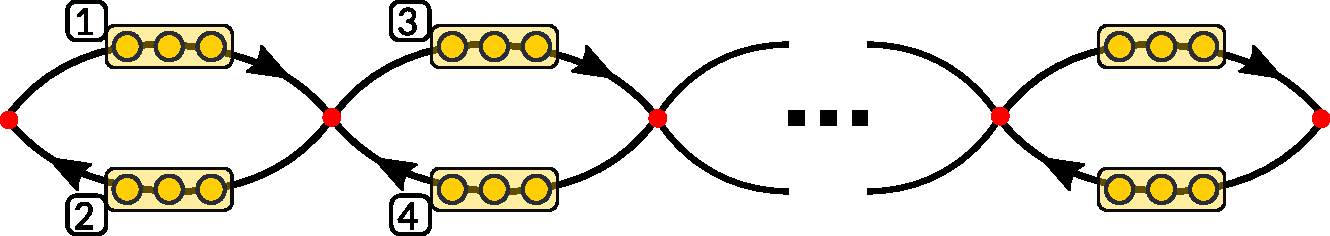
\includegraphics[width=\linewidth]{Figures/glasses.pdf}
    \vspace{0.05cm}
  %  \caption{Lattice}
    %\label{fig:gen_geom}
    \end{subfigure} %
    \hfill
    \begin{subfigure}{0.25\textwidth}
    \begin{equation*}
    \Qcircuit @C=0.2em @R=0.2em {
\lstick{m} & \gate{H} &       \ctrl{3} & \qw & \qw &\qw \\
\lstick{R} & \gate{H} &   \qw & \ctrl{3} & \qw & \qw \\
\lstick{R^{2}} & \gate{H} &  \qw & \qw & \ctrl{3} & \qw 
% \inputgrouph{1}{3}{2.2em}{\ket{h}}{2.5em}
\\
\lstick{\quad m} &  \qw &   \targ & \qw & \qw & \qw \\
\lstick{R} & \qw&   \qw &  \targ & \qw & \qw \\
\lstick{R^{2}} & \qw & \qw&   \qw &  \targ & \qw 
% \inputgrouph{4}{6}{2.2em}{\ket{g}}{2.5em}
}
\end{equation*}\vfill
    %\caption{Circuit}
  %  \label{figGS_prep}
\end{subfigure}
    \caption{Quasi one-dimensional lattice allowing for shallow ground state preparation of the quantum double model $D(D_4)$. Left: Yellow bars denote individual spins associated to edges, which are composed of three qubits each. Edge orientations are needed to define the vertex- and plaquette operators of the corresponding Hamiltonian and are drawn for the sake of concreteness. Right: Circuit for groundstate preparation per loop.}
    \label{fig:latticeGS}
\end{figure*}

%The ground state on this geometry, \caro{
%%I thought we always thought of this thing as being embedded in a sphere
%given an open boundary}, \caro{
%%it is entangled pairwise, it is not entangled along the chain
%is not entangled} and hence can be prepared in constant-depth.

The ground state on this geometry can be prepared in constant-depth.
Borrowing the notation from Figure \ref{fig:latticeGS}, we can write the ground state as:
\begin{equation}
    \ket{G.S.} = \sum_{\{g_{12}, g_{23}, \ldots\}} \ket{g_{12}}_1\ket{g_{12}}_2\ket{g_{34}}_3\ket{g_{34}}_4\ldots,
\end{equation}
where $\ket{g}_i$ is the state/label of the $i^{\text{th}}$ leg in Figure \ref{fig:latticeGS}.

The state in the above equation is not topologically ordered, in a sense that it does not have topological entanglement entropy.
However, one can build up the needed entanglement once one starts proliferating anyons via ribbon operators.
In fact, the geometry is robust enough to correctly represent the braiding statistics of the anyons, even if we must let ribbons touch due to size constraints, as long as they do not intersect.

The shallow circuit preparing this state is shown in Figure \ref{fig:latticeGS}.

We also examine fusion on a small two-dimensional graph, as shown in Figure \ref{fig:basketball}.

\begin{figure}
    \centering
    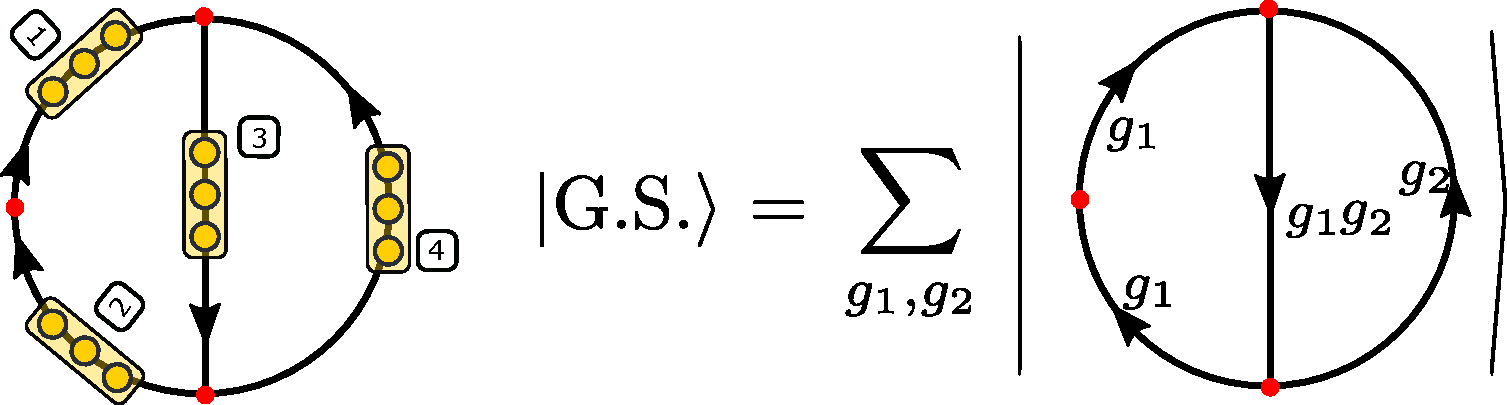
\includegraphics[width=\linewidth]{Figures/basketball.pdf}
    \caption{A small two-dimensional graph. Left: Yellow bars denote individual spins associated to edges, which are composed of three qubits each. Edge orientations are needed to define the vertex- and plaquette operators of the corresponding Hamiltonian and are drawn for the sake of concreteness. Right: The ground state on this small two-dimensional graph.}
    \label{fig:basketball}
\end{figure}


There has been a lot of work done in preparation of quantum double states on general graphs \cite{}.
These offer a constant depth protocols aided by measurements and error-correction.
However, for such simple and small graphs we opted to directly prepare the ground state using the general controlled group multiplication circuit, Table \ref{}, as well as Hadamard gate, see Figure \ref{}. \jovan{Where Caro stopped.}

\subsection{Anyon Fusion}

This is the simplest protocol.
It requires applying two ribbon operators between sites $s_1$ and $s_2$, and between sites $s_2$ and $s_3$, after preparing the ground state, naturally.
This creates two pairs of anyons and fuse then on site $s_2$, we then perform a reduced charge measurement and flux readout for this site.
This experiment is examined on both the braiding ladder and the two-dimensional small graph.
The protocol is shown on Figure \ref{}.

\todo{Figure Fusion: Showing the fusion experiment on two graphs.}

In principle, we can do this for any anyon type, but for concreteness we will choose the pure fluxes, $\Psi_m$, since the ribbon operator take a simple form for our choice of encoding, see Tables \ref{} and \ref{}.

They fuse as follows: $$\Psi_m \times \Psi_m = 0 + \tilde{0} + \Sigma_m + \tilde{\Sigma}_m,$$ $0$ being the vacuum, $\tilde{0}$ is the Abelian flux corresponding to the other element of the centre of $D_4$, $r^2$. The other two are pure charge associated with $\alpha_m$ representation of $D_4$ and the dyon of this pure charge and Abelian flux.

All four of these outcomes can be differentiated by reading out the flux and performing the $H_r$- or $H_{mr}$-reduced charge measurement. The $H_m$-reduced charge measurement doesn't see the difference between $0$ and $\Psi_m$.

The results of numerical for these two experiments are shown in Figure \ref{fig:fusion_glass} and \ref{fig:fusion_basketball}.

Here we see the four peaks corresponding to the four fusion outcomes for both geometries.
For further discussion of the numerical results, see Section \ref{sec:num}.

\subsection{Anyon Braiding}

The second phenomenological fact that gives the nonabelian anyons their name is the fact that the image of the braid group, as represented by physically braiding these anyons, is nonabelian. 
This means that the order of interchanges matter, i.e. $\sigma_{12}\sigma_{23} \neq \sigma_{23}\sigma_{12}$, where $\sigma_{ii+1}$ are clockwise interchange of particle $i$ and $i+1$, the generators of the braid group.

The braiding procedures we want to implement to show this fact are shown in Figure \ref{fig:flux_braid}.

\begin{figure}
    \centering
    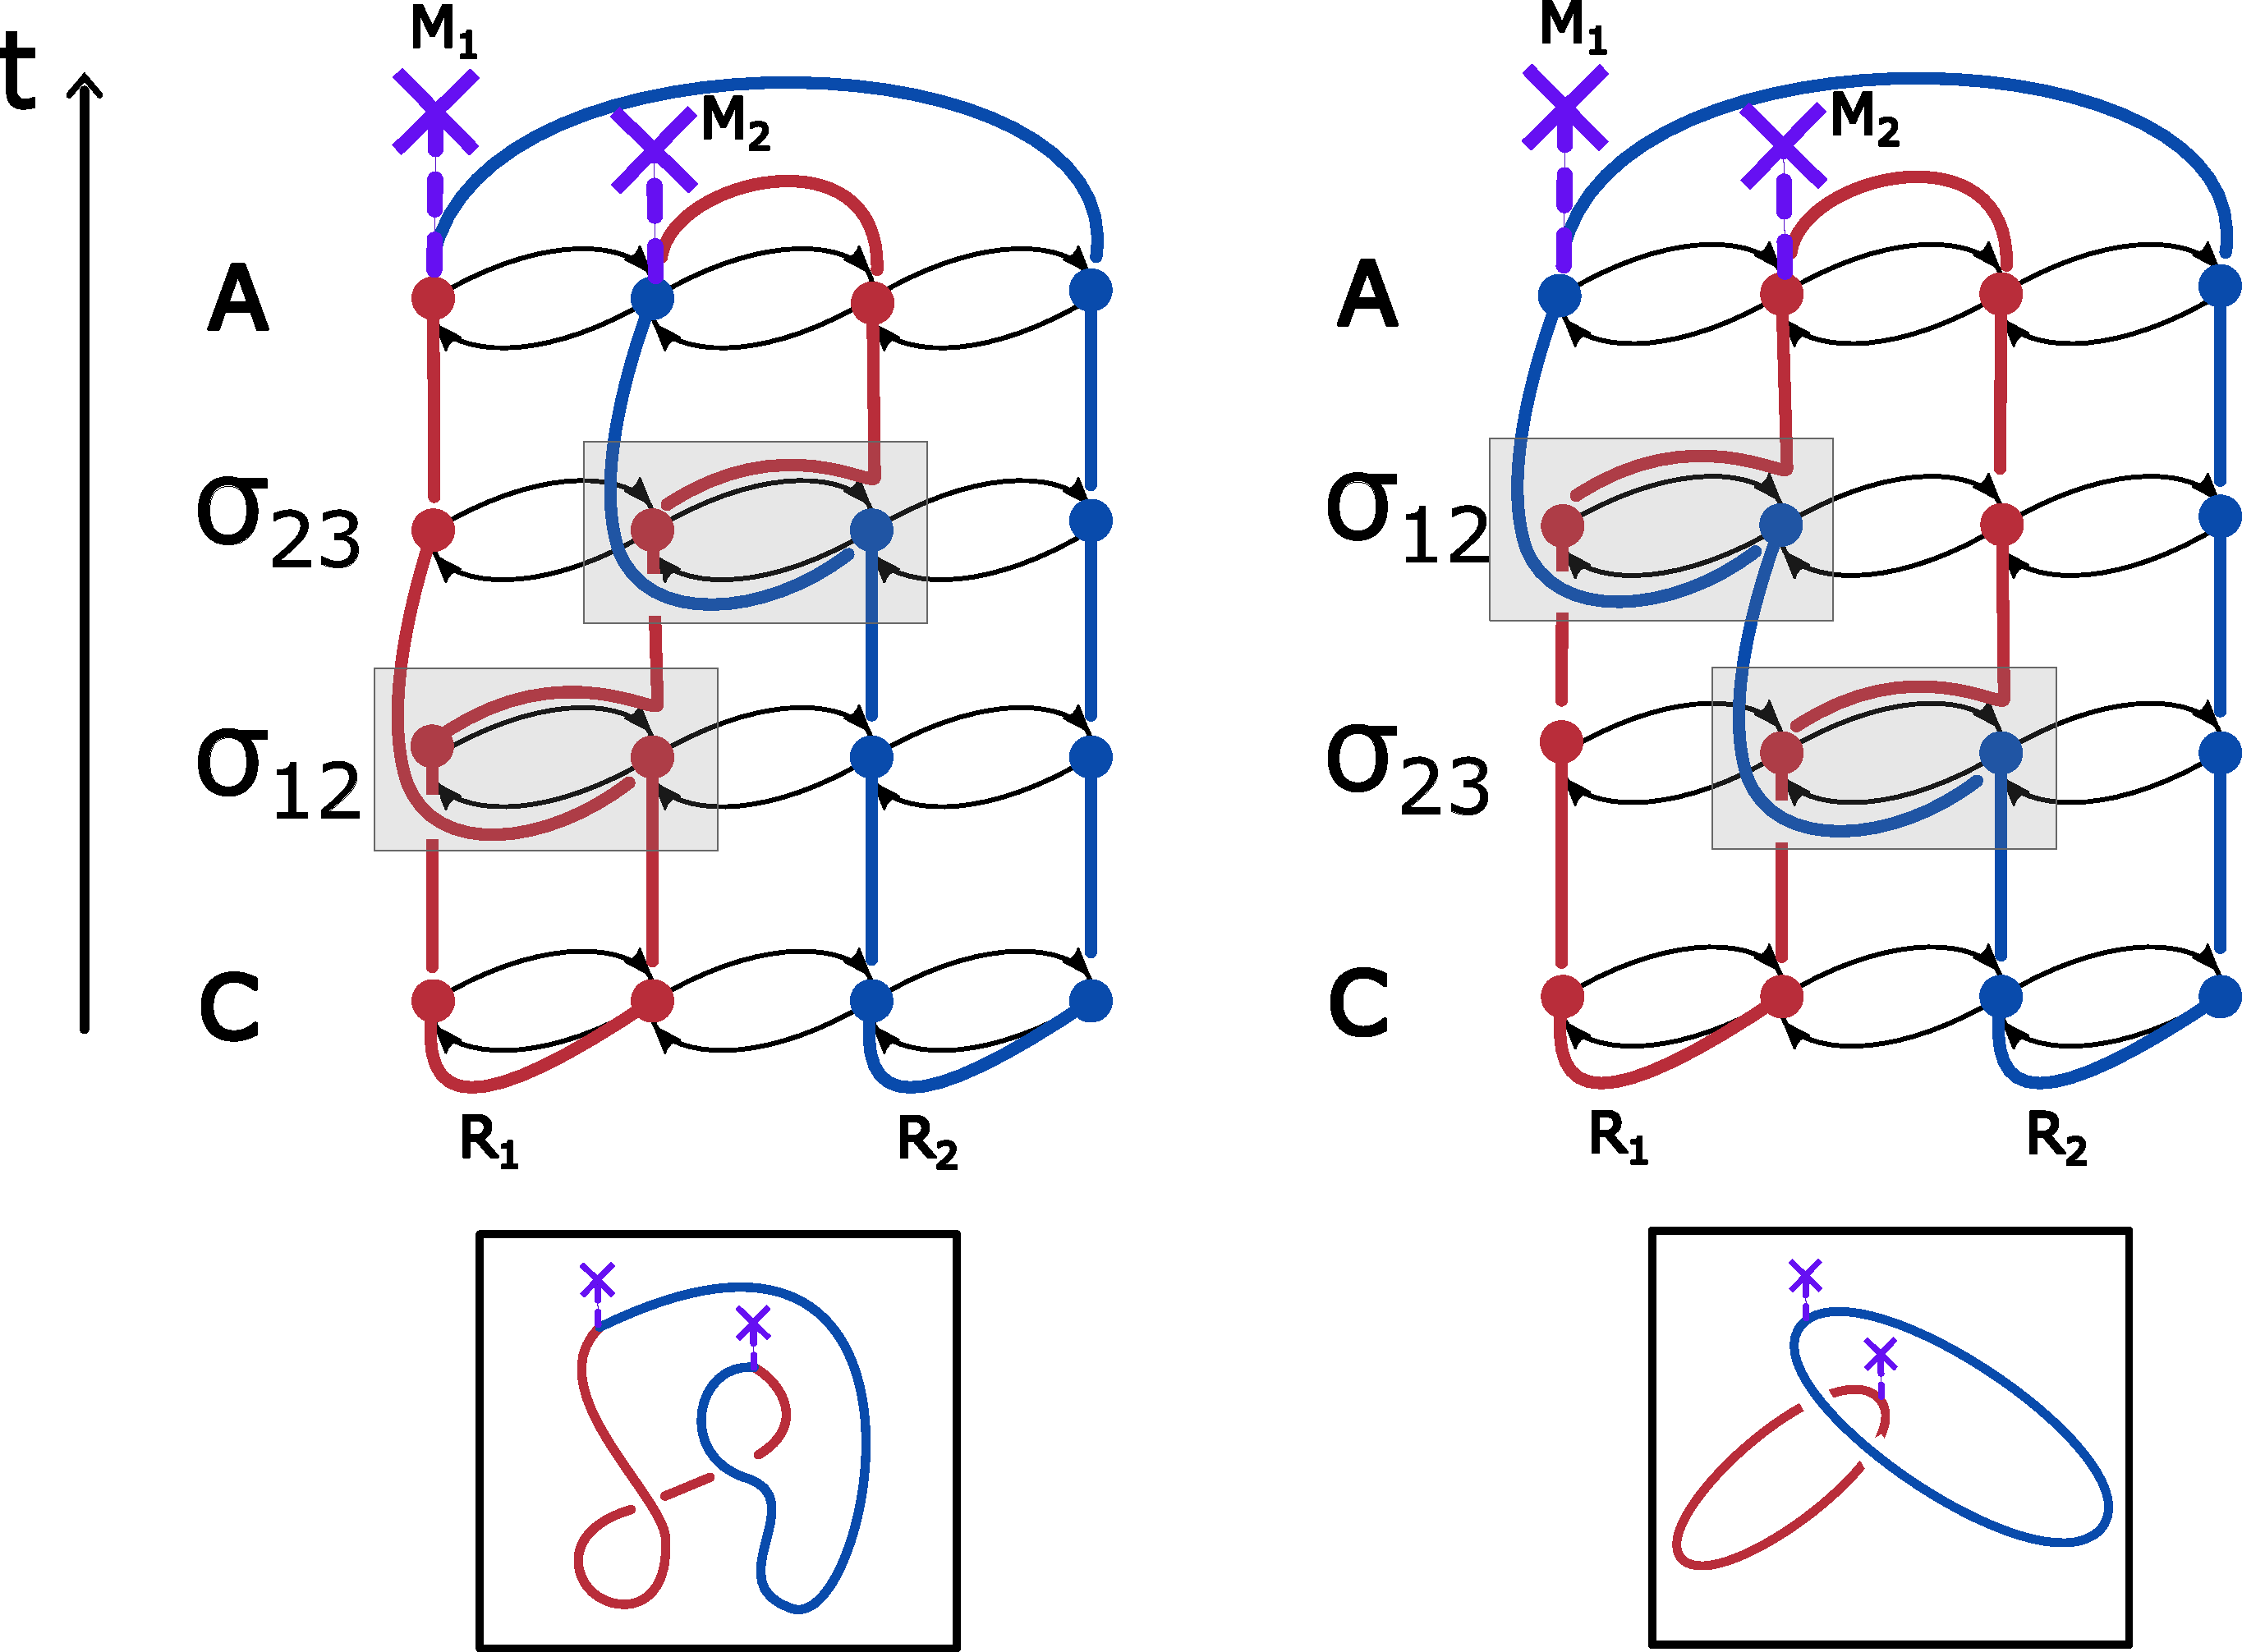
\includegraphics[width=\linewidth]{Figures/fluxBRAID.pdf}
    \caption{The two braiding protocols, differing only in order of exchange of two anyons. Protocol a) will have 4 fusion outcomes, while protocol b) can only produce vacuum.}
    \label{fig:flux_braid}
\end{figure}

Two pair of anyons are created from the vacuum, two interchanges are performed, and then the two pair are annihilated. 
In the first braiding, we annihilate the pairs that have a fixed fusion channel, given they are created from the vacuum they will fuse to the vacuum.
In the second braiding, we annihilate the pairs whose fusion channel is not fixed, hence all four outcomes are expected, the same result as in the fusion experiment.

The anyons we will braid are again pure fluxes $\Psi_m$, out of concreteness. The numerical results are shown in Figure \ref{fig:braid_fuse} and \ref{fig:braid_link}.

Here we see that the two braiding indeed produce two different states, the first is the vacuum and the second is a superposition of four possible fusion outcomes, as expected.
For further discussion of the numerical results, see Section \ref{sec:num}.

\begin{figure*}
\centering

\begin{subfigure}{0.47\textwidth}
    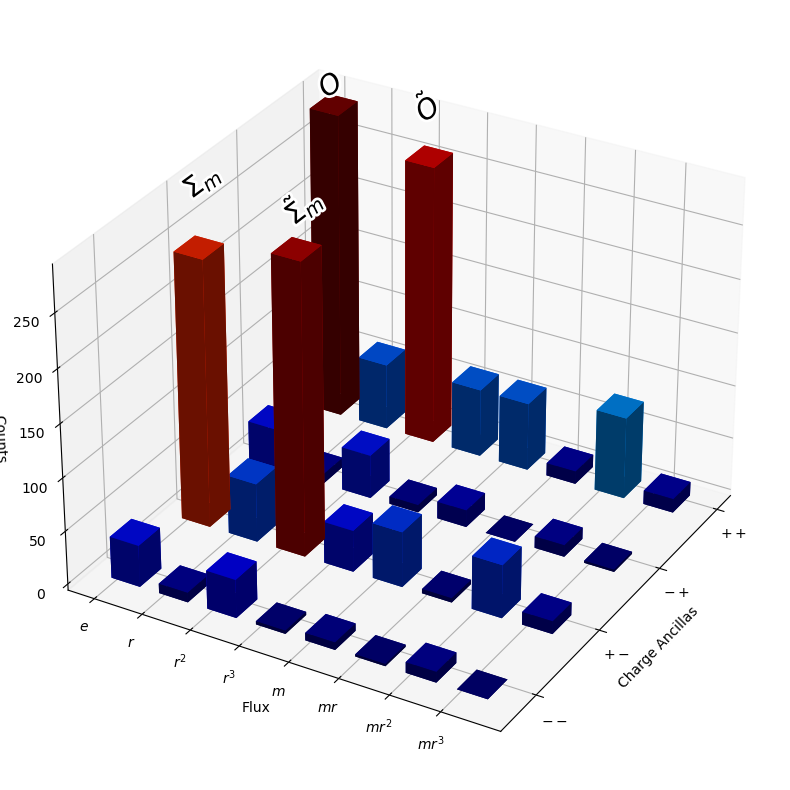
\includegraphics[width = \linewidth]{Figures/fusion_glasses.png}
    \caption{The reduced charge-flux measurement after fusing two $\Psi_m$ pure fluxes on the site of fusion. The reduced charge was done with $H_{mr}$ subgroup, and the geometry was that of the braiding ladder, Figure \ref{fig:gen_geom}.}
    \label{fig:fusion_glass}
\end{subfigure}\hfill
\begin{subfigure}{0.47\textwidth}
    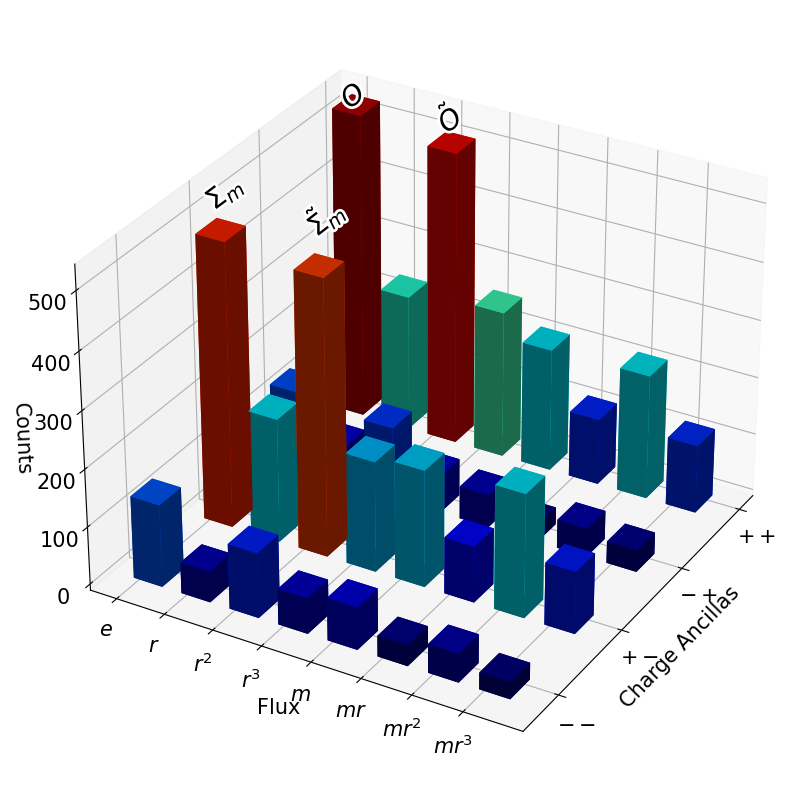
\includegraphics[width=\linewidth]{Figures/fusion_on_basketball.png}
    \caption{The reduced charge-flux measurement after fusing two $\Psi_m$ pure fluxes on the site of fusion. The reduced charge was done with $H_{mr}$ subgroup, and the geometry was that of the small two-dimensional graph, Figure \ref{fig:basketball}.}
    \label{fig:fusion_basketball}
\end{subfigure}
\vspace{15pt}

\begin{subfigure}{0.47\textwidth}
    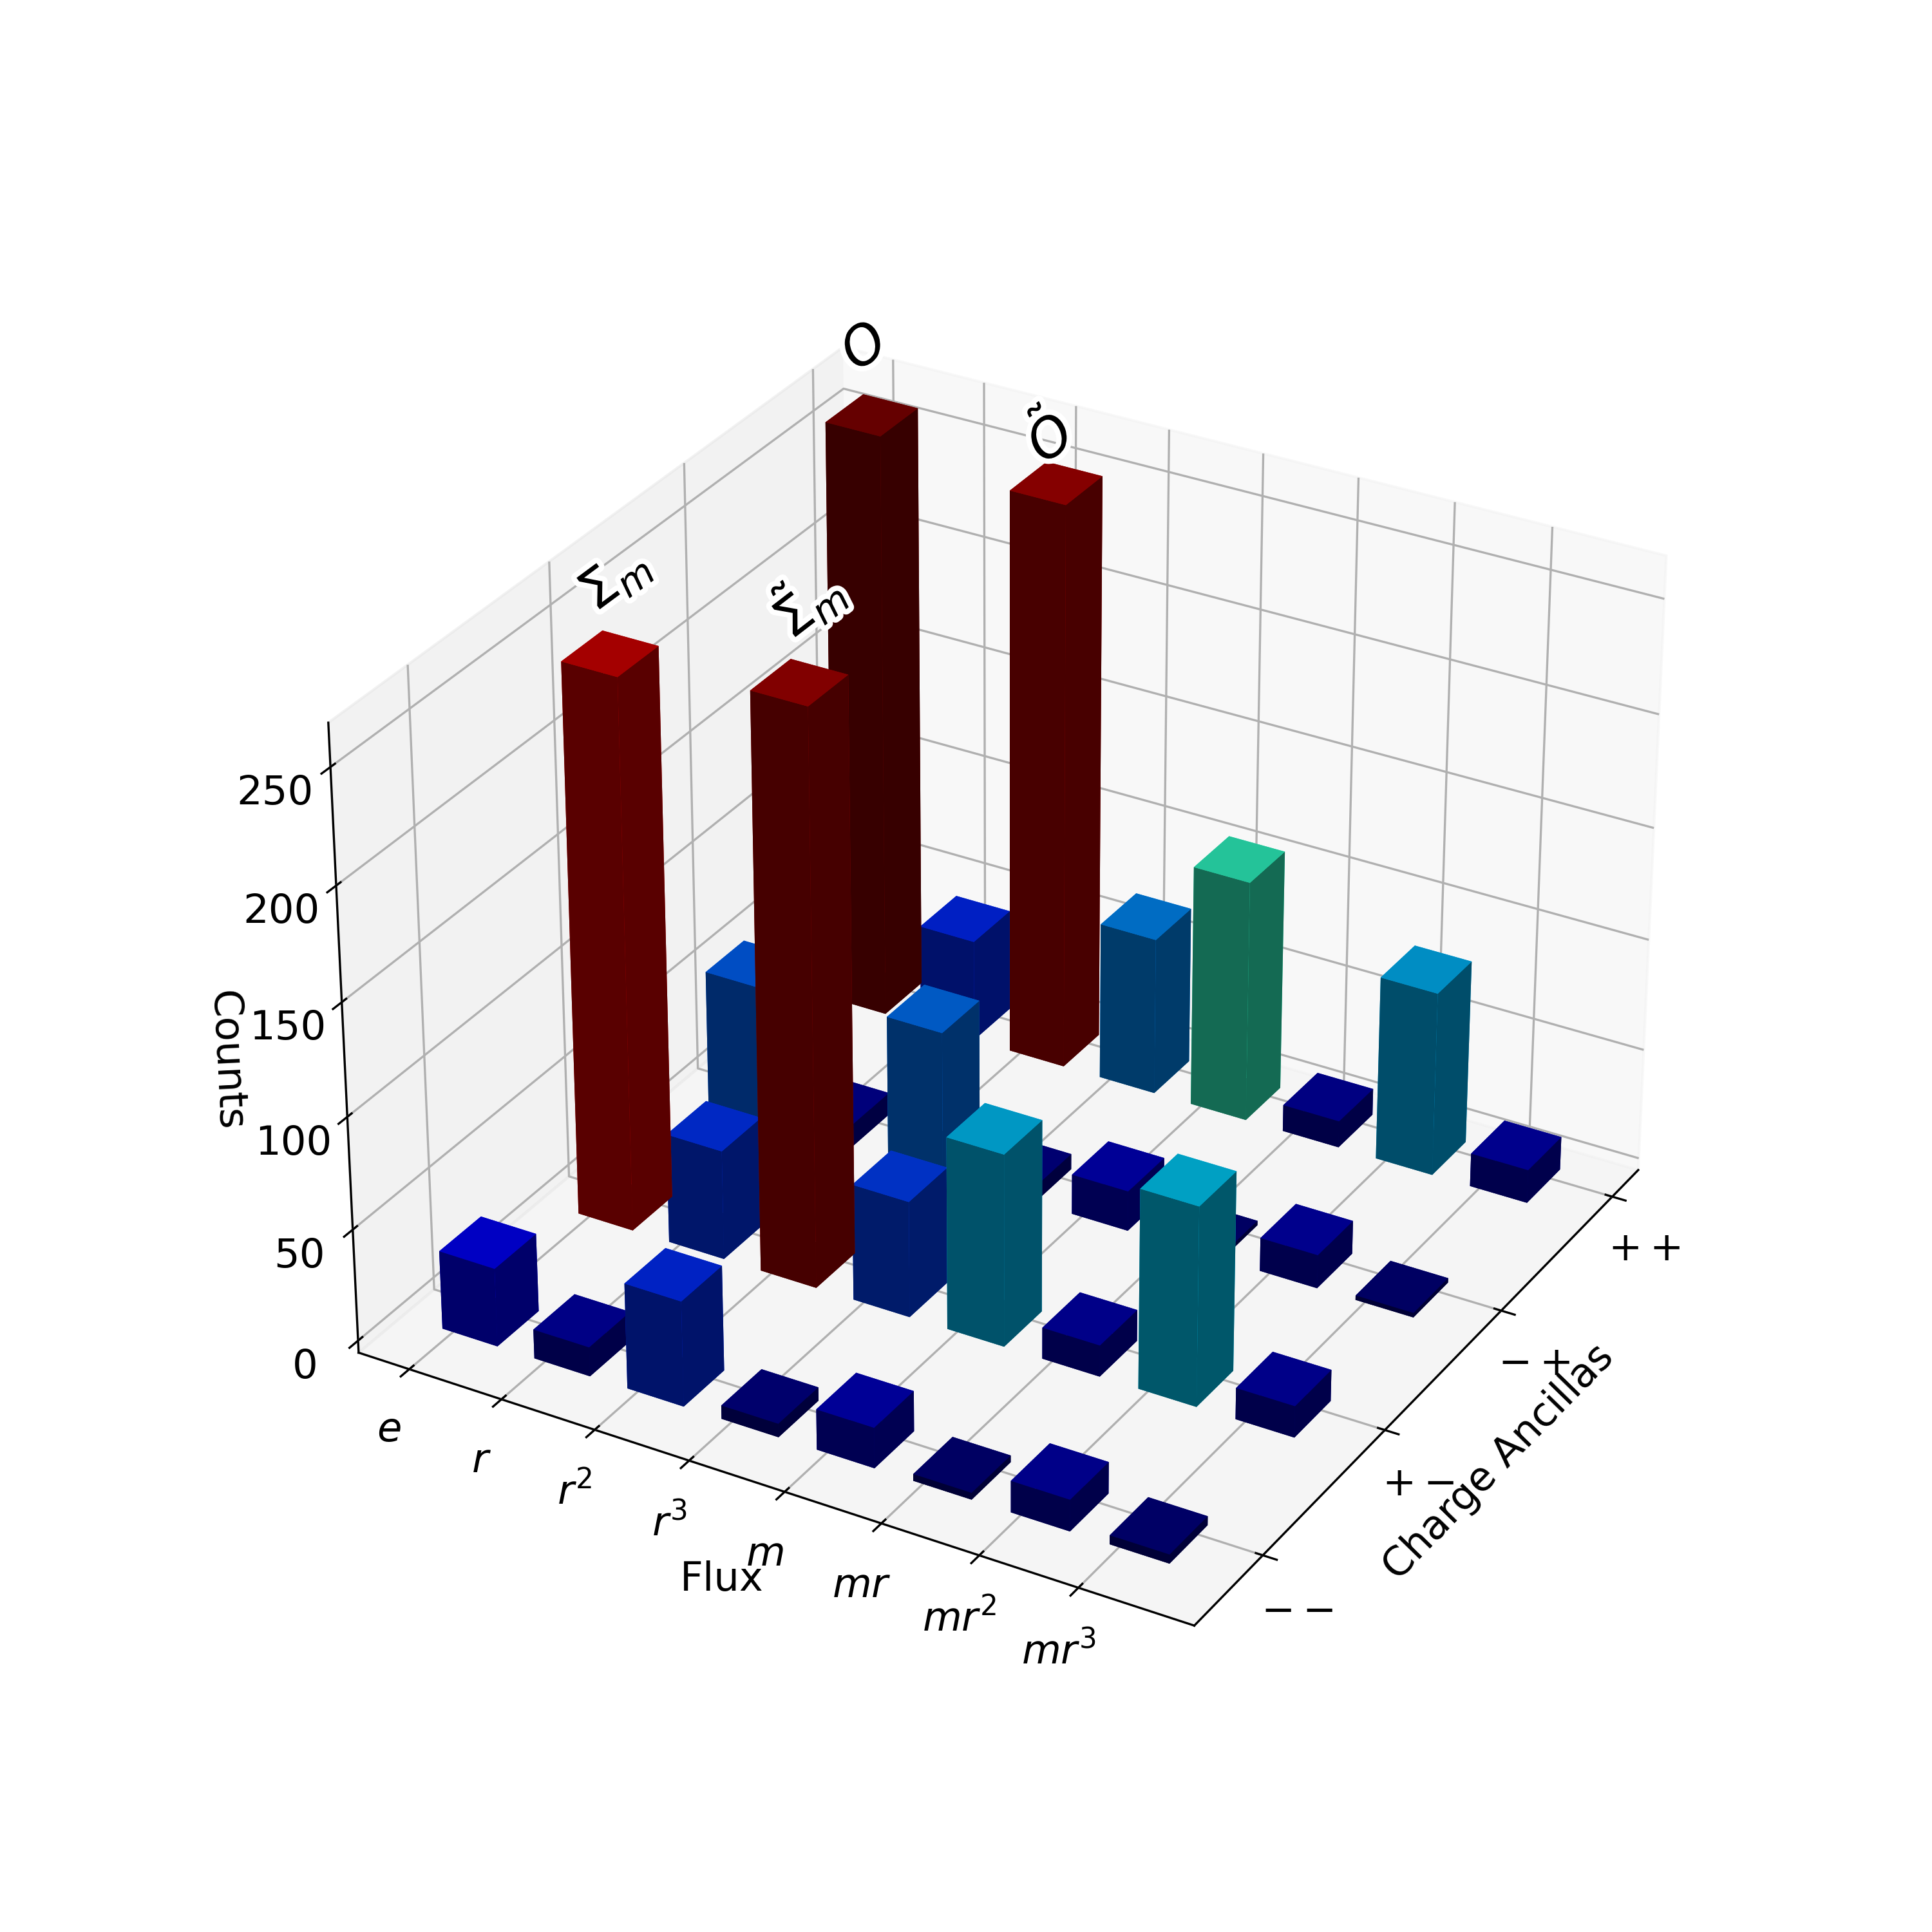
\includegraphics[width=\linewidth]{Figures/braid_fusion.png}
    \caption{The braiding on a braiding ladder: the reduced charge-flux measurement after performing the braiding protocol in $\sigma_{12}\sigma_{23}$ order, Figure \ref{fig:flux_braid} (left), where $\sigma_{ii+1}$ is a braid group generator. The anyons used are the pure fluxes $\Psi_m$. The reduced charge measurement was done with respect to $H_{mr}$ subgroup.} 
    \label{fig:braid_fuse}
\end{subfigure}\hfill
\begin{subfigure}{0.47\textwidth}
    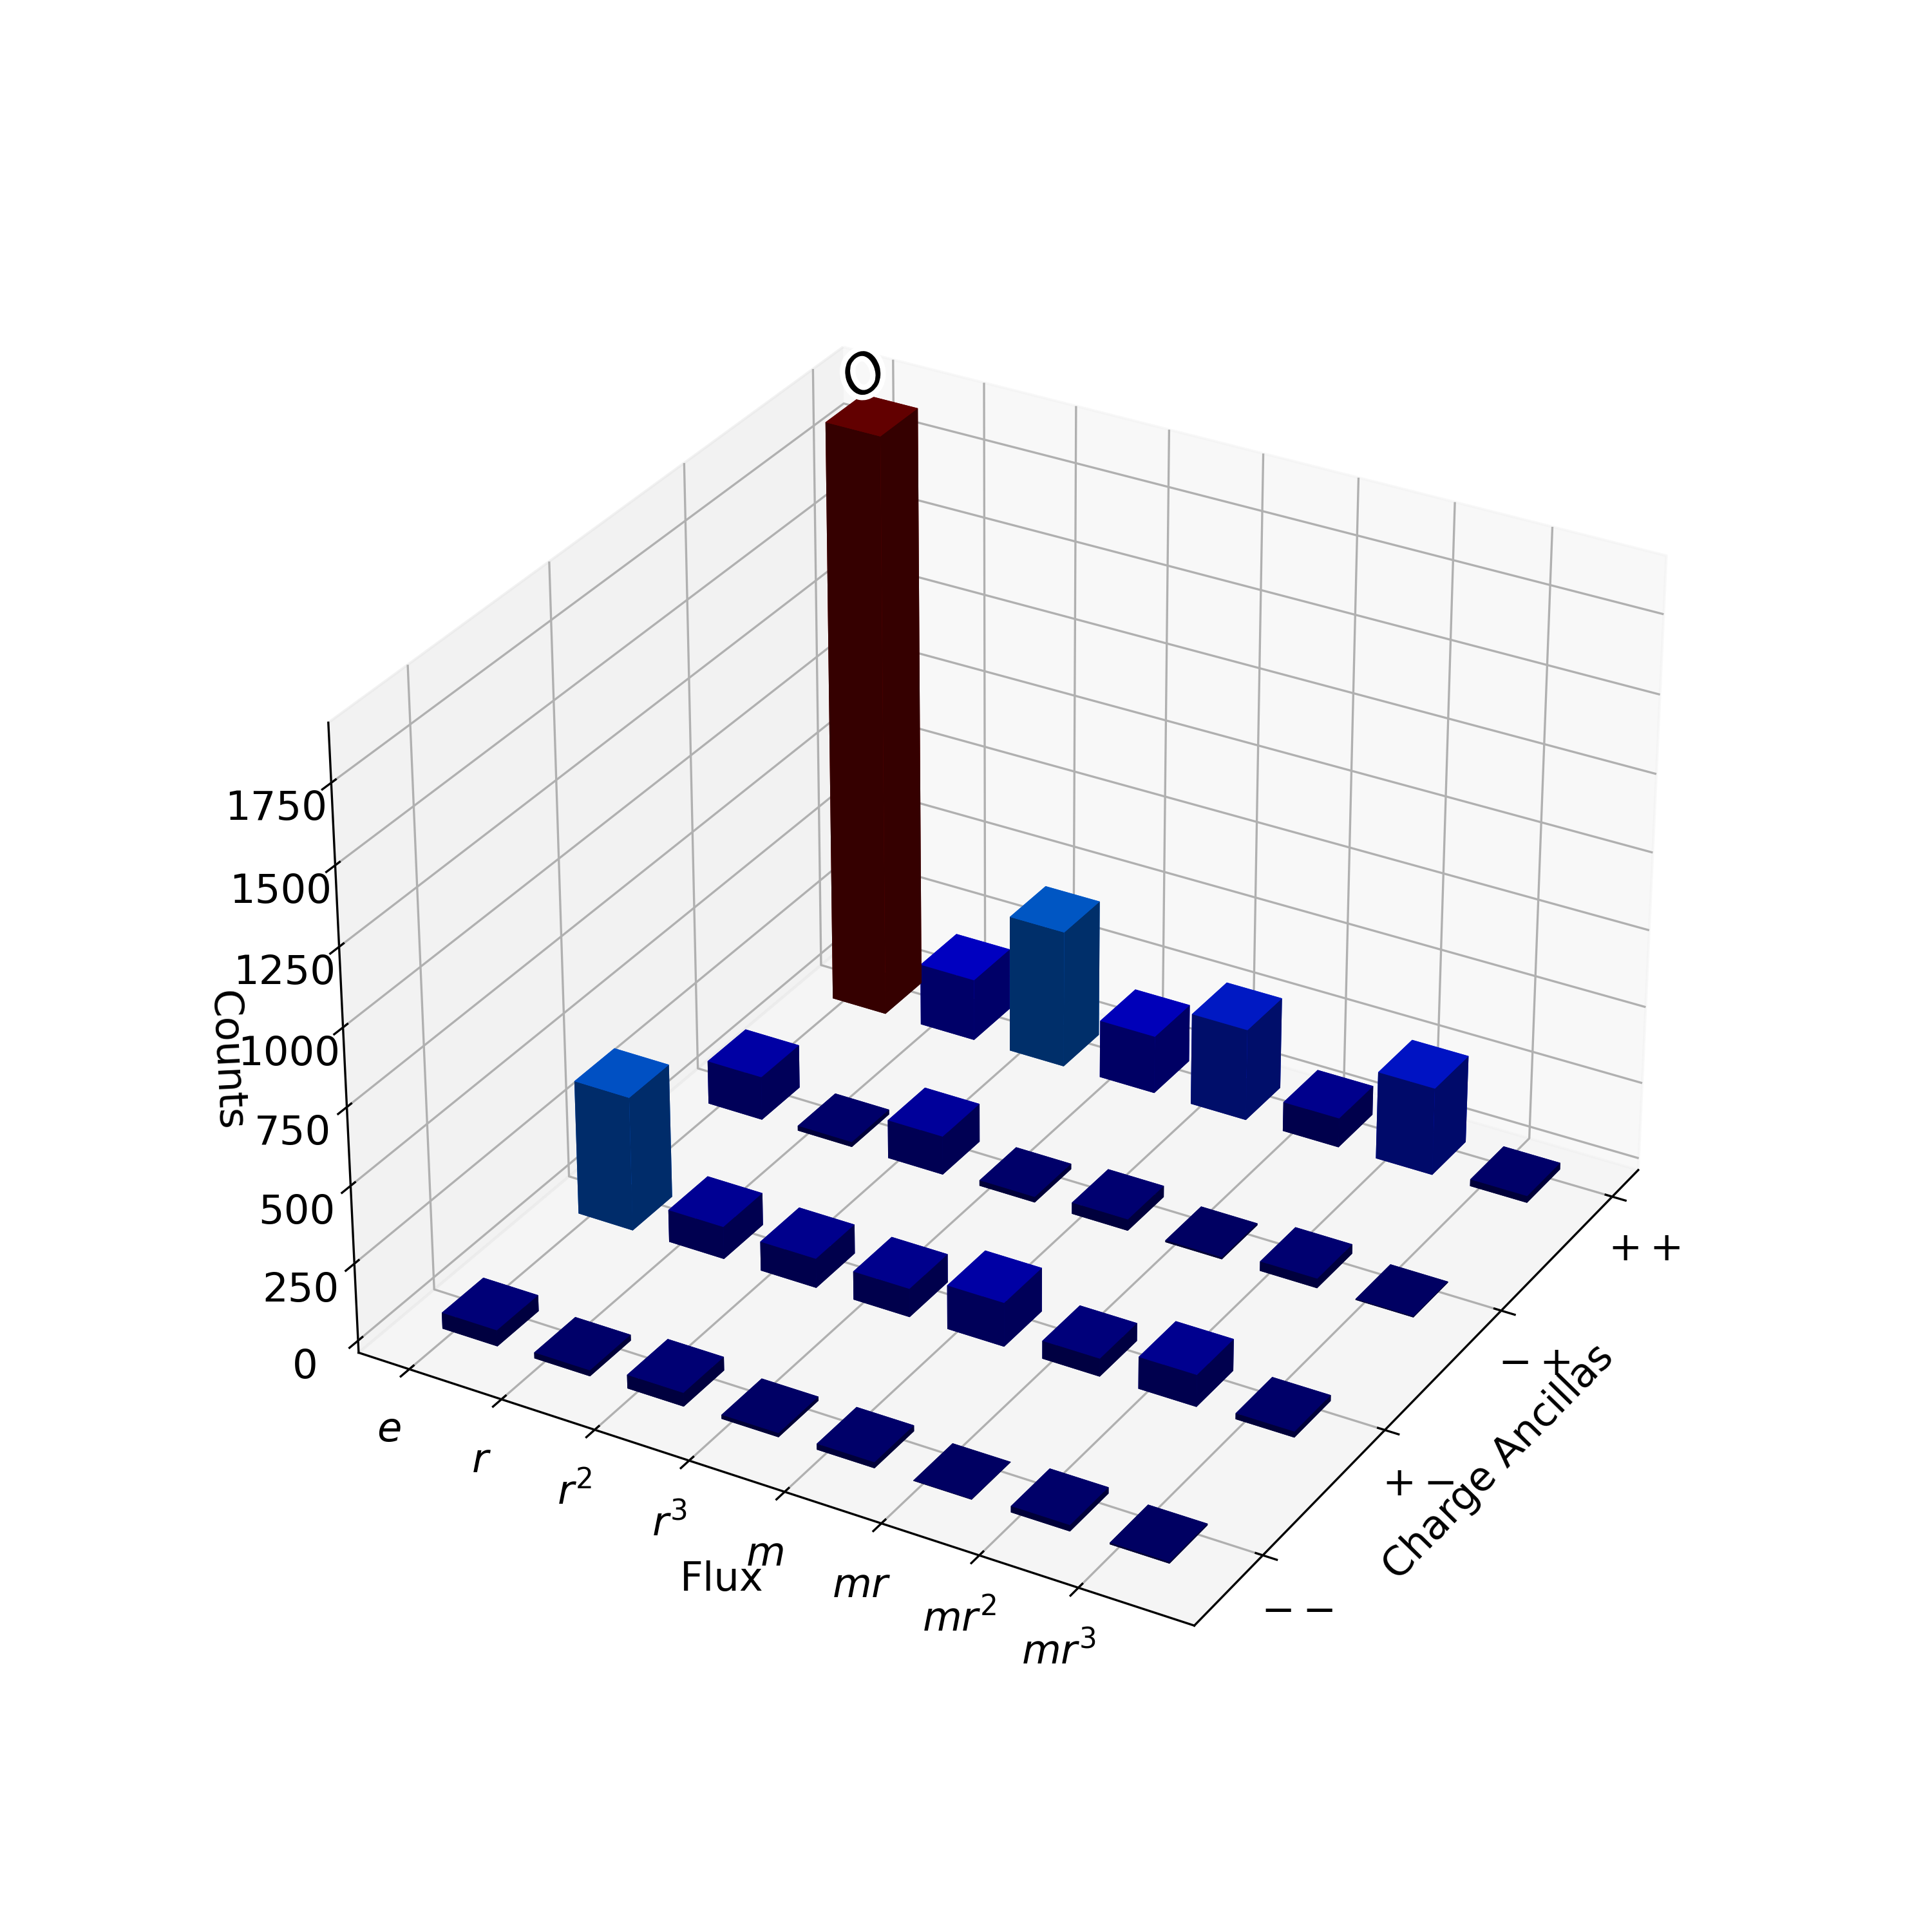
\includegraphics[width=\linewidth]{Figures/braid_link.png}
    \caption{The braiding on a braiding ladder: the reduced charge-flux measurement after performing the braiding protocol in $\sigma_{23}\sigma_{12}$ order, Figure \ref{fig:flux_braid} (right), where $\sigma_{ii+1}$ is a braid group generator. The anyons used are the pure fluxes $\Psi_m$.The reduced charge measurement was done with respect to $H_{mr}$ subgroup.}
    \label{fig:braid_link}
\end{subfigure}
\caption{The reduced topological charge measurements for the fusion and braiding protocols.}
\label{fig:red_charge_res}
\end{figure*}


\subsection{Interferometry}\label{subsec:Intef}

In order to access full data of the S- and T-matrix, amplitude and phase of its elements, we must devise an interference protocol.

There will be a controlling bit $c$, whose states are entangled with different braiding protocol after a specific protocol:
\begin{equation}
    \ket{\psi}_c\ket{\text{G.S.}} \rightarrow \ket{0}_c \ket{\Psi_0} + \ket{1}_c \ket{\Psi_1},
\end{equation}
where $\Psi_i$ are the two wave functions of the matter degrees of freedom corresponding to two braiding operations.

If the charge content of the two states is the same they may only differ by a constant, hence we can write:
\begin{equation}
    \ket{0}_c \ket{\Psi_0} + \ket{1}_c \ket{\Psi_1} = (\ket{0}_c + C_{01}\ket{1}_c)\ket{\Psi_0},
\end{equation}
and by the means of tomography on the control bit $c$ we can extract the relative constant $C_{01}$.

For a suitable choice of two braiding protocols, this constant can equal some element of S- (and T-) matrix, see Figure \ref{fig:intef_example}.

This superposition is constructed by conditional braiding, conditioned on the state of the control bit. 
The conditional braiding is achieved by applying conditional ribbon operators.
For example, we can condition the existence of a ribbon by making any unitary gate involved in applying the ribbon operator conditioned on the state of the control bit.
Every, single qubit gate becomes a two qubit gate and every two qubit gate becomes a three qubit gate (unitarily similar to a Toffoli gate), hence, the number of entangling gates grows fast.

A smarter alternative way is to condition the anyon flavour of the ribbon, a ribbon label that is. One just needs to look at two ribbon operators and identify where they differ, and condition only those operations. The result is illustrated in Figure \ref{fig:flavCond}.


\begin{figure}
\begin{equation*}
\begin{split}
\Qcircuit @C=0.5em @R=0.7em @!R{
\lstick{c} & \ctrl{1} & \qw\\
\lstick{m} & \targ & \qw \\
\lstick{R} & \qw  & \qw \\
\lstick{R^{2}} & \targ  & \qw \\
\lstick{\text{aux}} &  \ctrl{-1} & \qw
}\qquad\qquad
\Qcircuit @C=0.5em @R=0.7em @!R{
\lstick{c} & \ctrl{3} & \qw& \ctrl{1}& \qw\\
\lstick{m} & \qw & \qw & \targ& \qw\\
\lstick{R} & \qw  & \qw & \qw& \qw\\
\lstick{R^{2}} & \targ  & \qw & \qw& \qw\\
\lstick{\text{aux}} &  \ctrl{-1} & \qw& \qw& \qw
}\qquad\qquad
\Qcircuit @C=0.5em @R=0.7em @!R{
\lstick{c} & \ctrl{2} & \qw\\
\lstick{m} & \qw & \qw \\
\lstick{R} & \ctrl{2}  & \qw \\
\lstick{R^{2}} & \qw  & \qw \\
\lstick{\text{aux}} &  \targ & \qw
}
\end{split}
\end{equation*}
\caption{The compiled conditional ribbon operators, where the flavour of the ribbon is conditioned on the state of the control bit $c$. Left: controlled multiply circuit used when anyon moves along a leg $i$ encoded by the middle three bits, control bit $c$ selects between pure flux $\Psi_m$ and reducible label $0\oplus\tilde{0}$. Center: controlled multiply circuit used when anyon moves along a leg $i$ encoded by the middle three bits, control bit $c$ selects between pure flux $\Psi_m$ and reducible label $0\oplus 0$, i.e. doing nothing. Right: controlled conjugation circuit used when anyon crosses along a leg $i$ encoded by the middle three bits, control bit $c$ selects between pure flux $\Psi_m$ and reducible label $0\oplus\tilde{0}$ or $0\oplus 0$. Note: ribbons can also be associated with reducible representations of $D(G)$ as long as they are closed, if we require a well-defined topological charge of the end state, the scheme for applying ribbon operators associated with the reducible representations is the same as for the irreducible representations.}
\label{fig:flavCond}
\end{figure}

In that example, the control bit is selecting between two ribbon flavours, the pure flux $\Psi_m$ and the one labelled by a reducible two-dimensional representation $0 \oplus \tilde{0}$. One can also look at the case where we condition the existence of the ribbon, by making every gate controlled by qubit $c$, as also selecting between two flavours, $\Psi_m$ and $0 \oplus 0$, the previous scheme simplifying the multiplication past of the circuit, Figure \ref{fig:flavCond} (left).

We will use both schemes in our phase-sensitive S-matrix experiment.

\subsubsection{S-matrix elements}

In this section, we describe in detail the inference protocols for measuring the S-matrix element.
The two protocols are based around conditional ribbon operators.
We explore two options when it comes to conditional ribbon operators.

First, depending on the state of some control qubit, $c$ the flavour of the ribbon is either some well-defined anyon label $b$, well-defined meaning $b$ is an irrep of $D(D_4)$, or a reducible representation $0\oplus\tilde{0}$ spanned by vectors $\{\ket{e;1}, \ket{r^2;1}\}$.
The ribbon operator application scheme is the same for ribbons labelled by reducible and irreducible representations.

Second, depending on the state of the control bit $c$, the flavour is either $b$ or $0\oplus 0$. This basically means that if the state of the control is $\ket{0}_c$ then we do nothing.

The second method, shown in Figure \ref{fig:cond_ex} in conjunction with the calibration shown in Figure \ref{fig:phase_check},  is conceptually the same as the ideal protocol in Figure \ref{fig:intef_example}. 
The calibration is done to make sure there is no dynamical phase accumulated by applying the $b$ ribbon by itself.

However, given every operation of the conditioned ribbon is conditioned on $c$, the complexity of the circuit for the second option is bigger than the first option where only some operations are conditioned on $c$.

The first method shown in Figure \ref{fig:cond_flav} is, as a quantum circuit, much simpler than the second method. 
However, it requires some input from the theory, that being $S(a, 0)$ and $S(a, \tilde{0})$ which in fact can be directly measured with a very simple protocol since $0$ and $\tilde{0}$ are Abelian, see Appendix \ref{app:abl}.

If $S(a, 0) = S(a, \tilde{0}) = 1$, then the factorization presented in Figure \ref{fig:cond_flav} is correct, and we can just read off the $S(a,b)$ after tomographing the control bit.

Note that the S-matrix appearing in Figure \ref{fig:S-mat} is normalized:
\begin{equation}
    \tilde{S}(a,b) = \frac{|D_4|}{d_a d_b}S(a,b),
\end{equation}
which makes $|\tilde{S}(a,b)| \leq 1$.

In our example, we will fix $b$ to be pure flux $\Psi_m$ again due to the relative simplicity of its ribbon operators. For the other anyon we will choose one of the following $a\in\{\Psi_m,\tilde{\Psi}_m, \Phi_r \}$ which gives us all three possible values of the S-matrix elements for the $D_4$ theory, those being $\{1, -1, 0\}$ respectively.

The exact method of tomography we will use will be presented alongside the numerical result, Figure \ref{}, in Section \ref{sec:num}. The way the noise interact with the protocol is non-trivial and deserves a separate discussion.

\begin{figure*}
\centering

\begin{subfigure}{0.47\textwidth}
    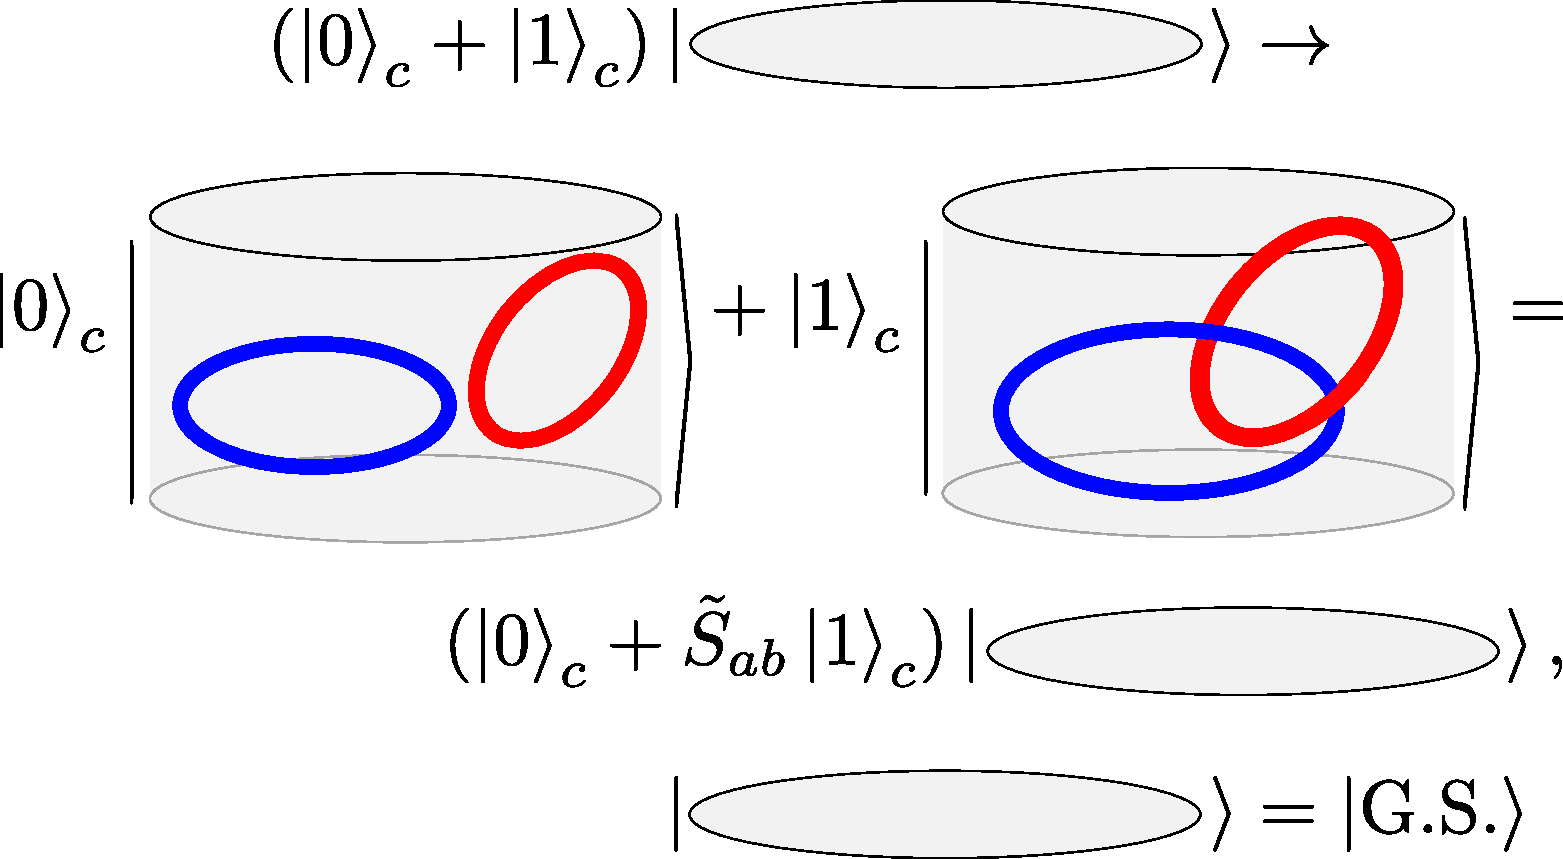
\includegraphics[width = \linewidth]{Figures/intef_example.pdf}
    \caption{The ideal interferometry scheme for measuring the S-matrix elements. The two possible braiding are appropriately entangled with the controlling bit $c$, which is achieved by controlled ribbon operators.}
    \label{fig:intef_example}
\end{subfigure}\hfill
\begin{subfigure}{0.47\textwidth}
    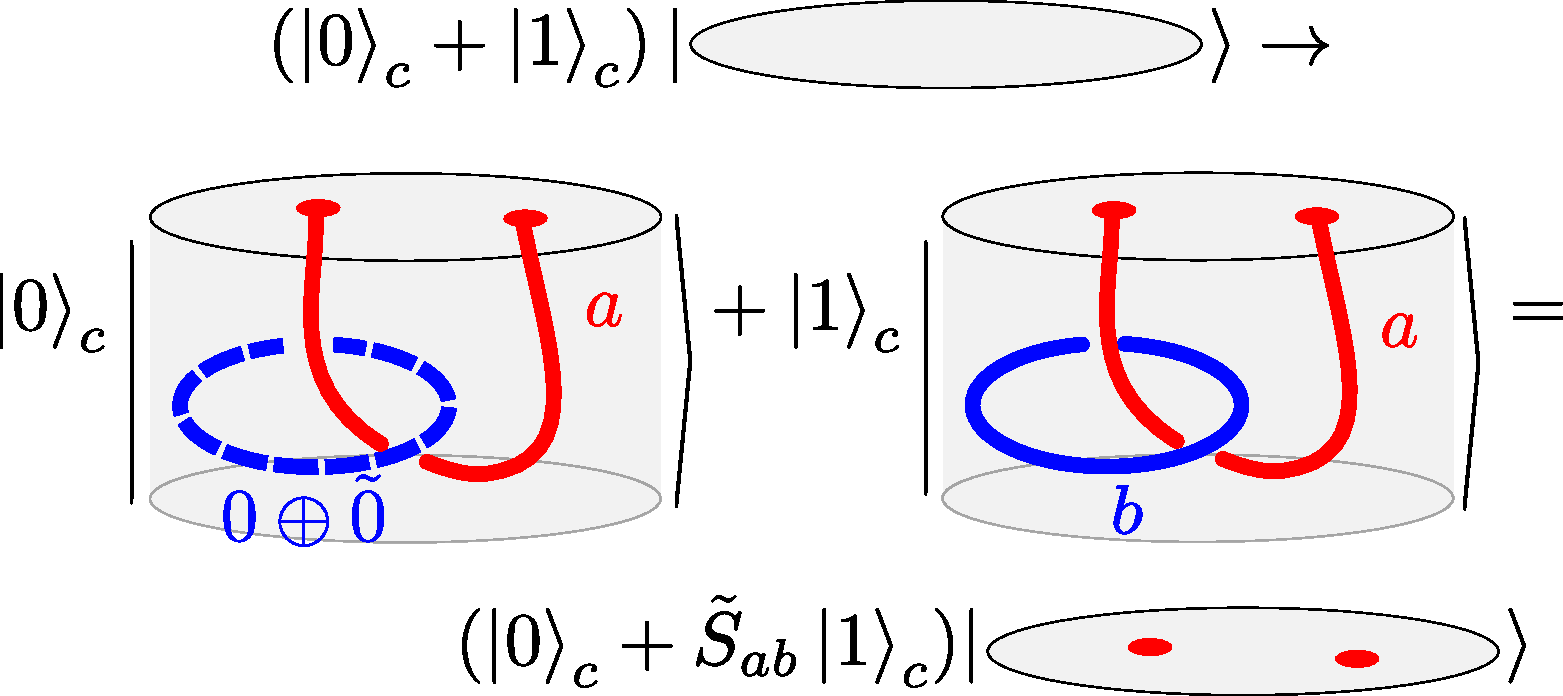
\includegraphics[width=\linewidth]{Figures/intefFlav.pdf}
    \caption{Conditioning the flavour of the ribbon, if the state of the control bit is $\ket{0}_c$ then the flavour is the reducible representation $0\oplus\tilde{0}$ and $\Psi_m$ otherwise. This is the shallowest protocol in terms of total compiled circuit depth.}
    \label{fig:cond_flav}
\end{subfigure}
\vspace{15pt}

\begin{subfigure}{0.47\textwidth}
    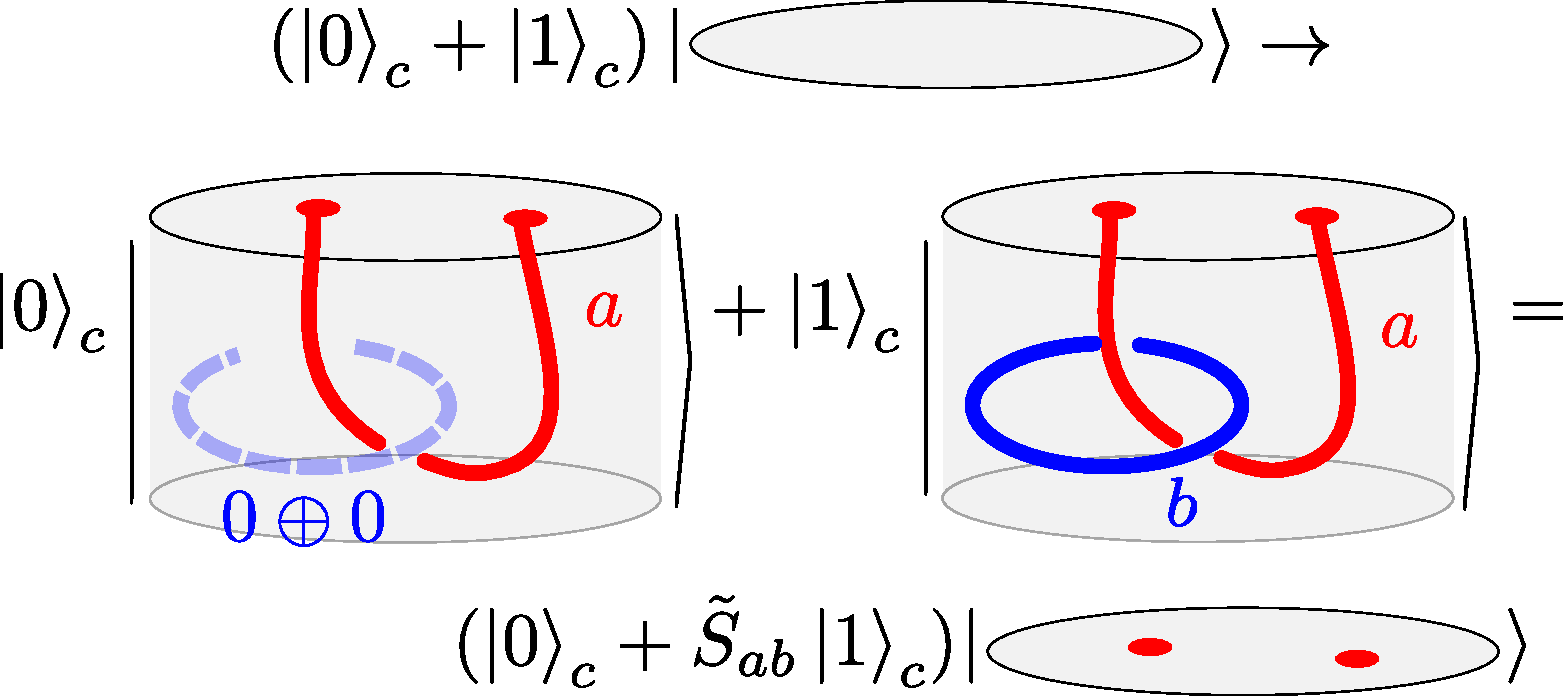
\includegraphics[width=\linewidth]{Figures/intefEx.pdf}
    \caption{Conditioning the existence of the ribbon, if the ribbon $\Psi_m$ is only applied if the state of the control bit is $\ket{1}_c$. You can also look at it as flavour conditioning, where the other flavour is the reducible $0\oplus 0$.}
    \label{fig:cond_ex}
\end{subfigure}\hfill
\begin{subfigure}{0.47\textwidth}
    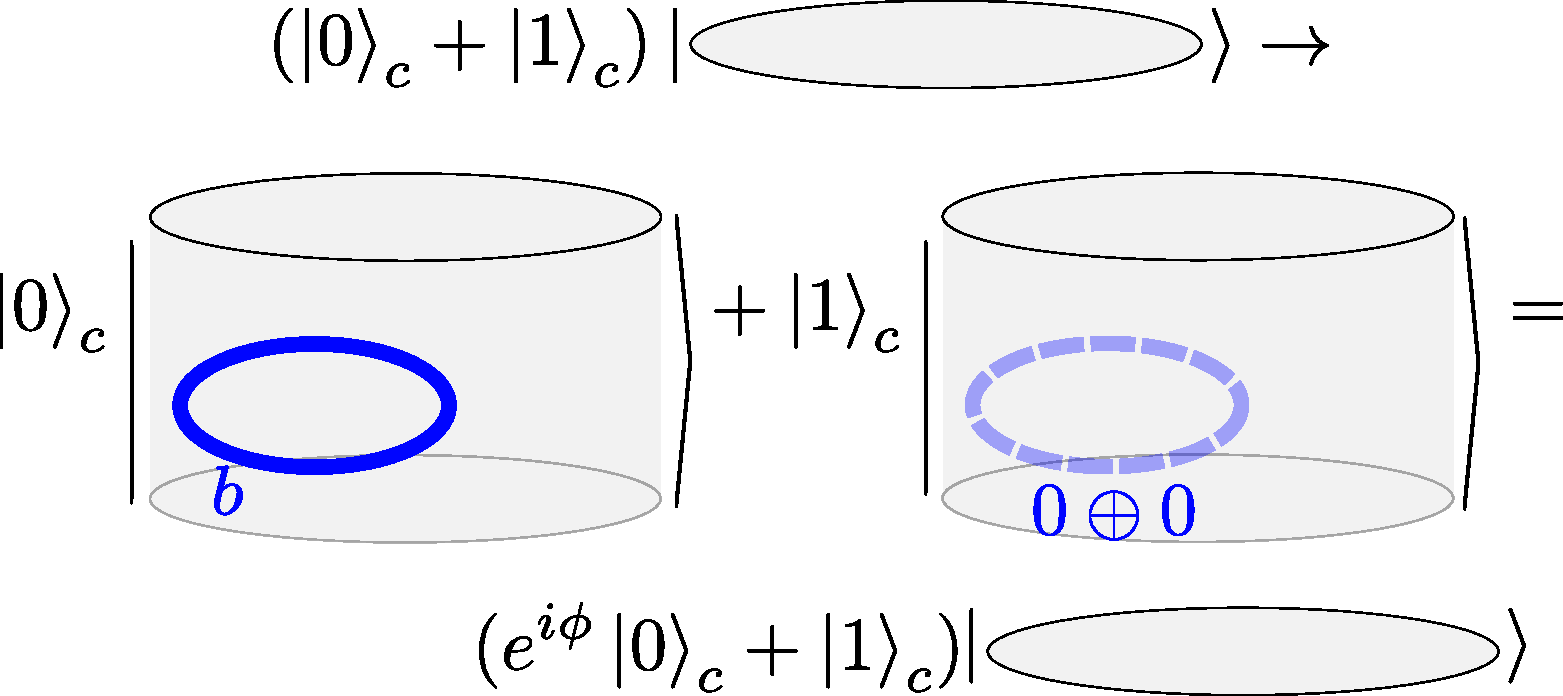
\includegraphics[width=\linewidth]{Figures/phaseCheck.pdf}
    \caption{Phase check. Making sure to remove any phase that is due to the application of the closed ribbon $\Psi_m$ itself.}
    \label{fig:phase_check}
\end{subfigure}
\caption{The interference protocols used in the numerical simulation for phase sensitive measurement of following S-matrix elements $S(a, \Psi_m)$ for $a\in\{\Psi_m, \tilde{\Psi}_m, \Psi_r\}$.}
\label{fig:S-mat}
\end{figure*}

\begin{figure*}
\centering
\begin{subfigure}{0.47\textwidth}
    \centering
    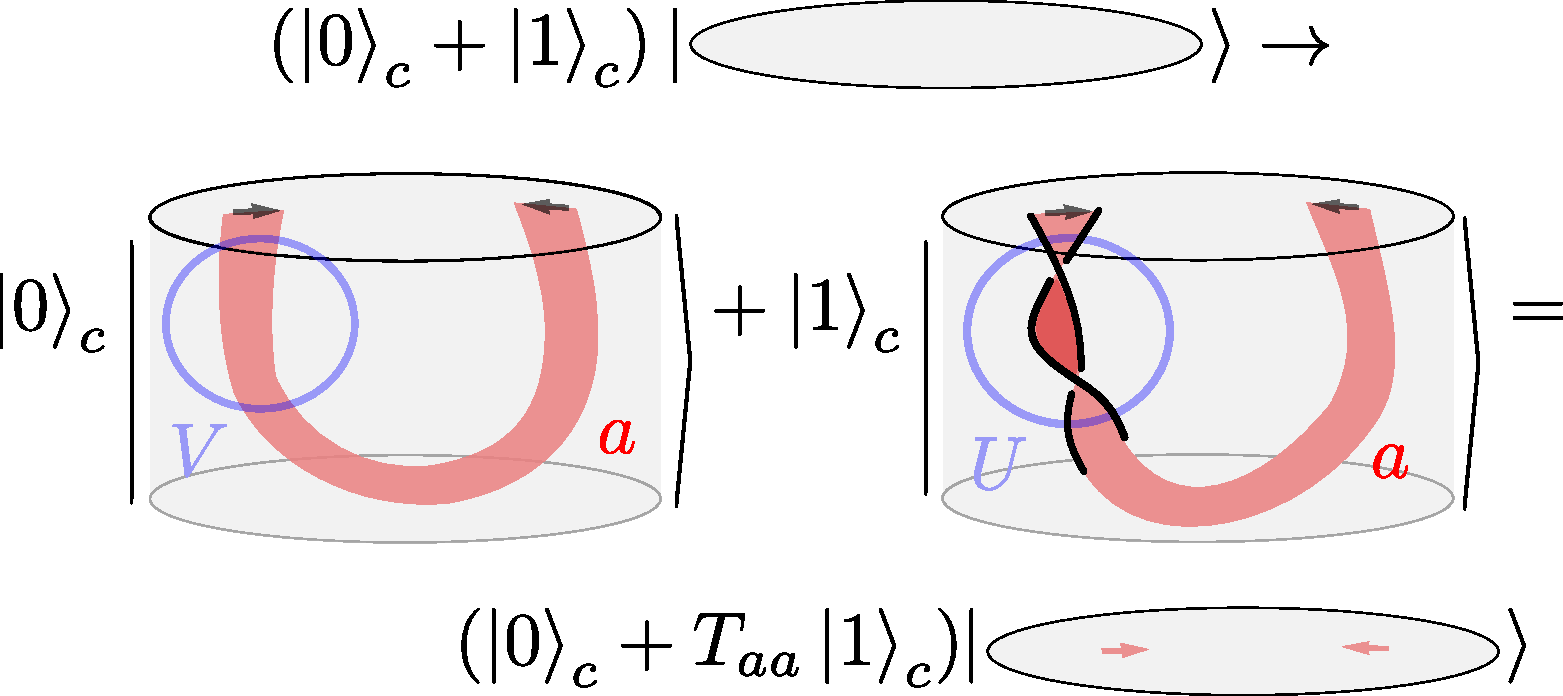
\includegraphics[width = \linewidth]{Figures/Tmat2.pdf}
    \caption{Interference protocol for measuring the phase of the T-matrix elements. Note: $|T_{aa}| = 1$ for all anyons $a$. The inference is done between two paths that differ by only one twist. We have restored the two-dimensionality of the ribbons in our representation in order to showcase the extra twist.}
    \label{fig:Tmat}
\end{subfigure}\hfill
\begin{subfigure}{0.47\textwidth}
\begin{equation*}
\Qcircuit @C=0.5em @R=0.7em @!R{
\lstick{c}&\qw&\ctrl{1}&\qw& \gate{X}&\qw&\ctrl{1}&\qw&\gate{X}&\qw\\
\lstick{\text{aux}}&\qw&\multigate{1}{U}&\qw &\qw&\qw&\multigate{1}{V}&\qw&\qw&\qw\\
\lstick{G.F.}&\qw&\ghost{U}&\qw&\qw&\qw&\ghost{V}&\qw&\qw&\qw
}
\end{equation*}
\caption{A circuit that depending on the state of the control bit $c$ either applies a unitary $U$ or $V$ onto the joint gauge field ($G.F.$) and auxiliary (aux) degrees of freedom.}
\label{fig:condcirq}
\end{subfigure}
\caption{The interferometry scheme to measure the phase difference between two paths alongside with a circuit diagram implementing the difference of the two paths.}
\label{fig:tmatfull}
\end{figure*}



\subsubsection{T-matrix elements}

In this section, we will describe the interference protocol for measuring the matrix elements of the diagonal T-matrix, or the spin of the anyons.
Here we note that ribbon operators are in-fact ribbons in space-time, hence they can acquire a twist.
Each twist contributes a phase factor to the wavefunction, $T_{aa} = e^{i\theta_a}$, just like the electron's wavefunction acquires a $\pi$-Barry phase once we take its spin around a great circle on a unit shere once.
In 2+1 dimensions the phases are not restricted to $0$ and $\pi$, for example $\pi/2$ in the case of some anyons of $D_4$ theory.

The protocol is illustrated in Figure \ref{fig:Tmat}.

The way we realize this interference scheme is as follows.
We identify where the two paths differ and apply a usual ribbon operator associated with some anyon $a$. Where they differ, we apply a controlled circuit of the form illustrated in Figure \ref{fig:condcirq}.

In Figure \ref{fig:condcirq} we have that unitary $U$ applies a ribbon operator along one path and $V$ along another one, in order to get the wavefunction in Figure \ref{fig:Tmat}.

The endpoint of the two ribbons are on the same site, hence the charge contetnt is the same, we can factor out the Gauge Field wavefunction. 
The control bit in the pure state that we can tomograph and read off the twisting phase.
The process of the tomography in this case is a bit elaborate, given the nontrivial way the noise play a part in this, hence we will leave the discussion of the results, Figure \ref{}, for Section \ref{sec:num}.

\section{Numerical Experiments}\label{sec:num}

In this section, we provided numerical evidence for the feasibility of our proposal, i.e. a set of noisy quantum circuit simulations that show that the nonabelian braiding signatures are observable.

The simulations were done via Google's 'cirq\_google' python package running on Google's cloud computing platform 'Google Colab'. This package executes the quantum trajectory simulation of the circuit using the Kraus operators obtained from the direct Pauli Transfer Matrix tomography on various single and two qubit gates on the Sycamore chip \cite{}.

Knowing the characteristics of the two-qubit gates, single-qubit gates and single- and multi-qubit readout performances of the chip \cite{} we have chosen a suitable part of the chip for our numerics, a similar setup would be suitable for an actual experiment if it to be done on the Sycamore chip, however, the optimal allocation of recourses (gauge field degrees of freedom, ribbon ancillaries, control and other) will be chip depended. The layout we used is shown in Figure \ref{}.

Given that we argue for feasibility of these experiments, i.e. will the signals we expect be detectable given the noise, we have to take into account how well does this numerical scheme, quantum trajectories with noisy one- and two-qubit gates, will reproduce the actual measurements.

Heuristics shows that it is in fact a good approximation of what we expect to see from the actual experiment \cite{}, even if it neglects any cross-talk between qubits that are not directly coupled by the circuit.

It is also important to note that, further to the size limitation imposed by the chip, we are further limited by the number of qubits we can simulate classically.
Indeed, for the case of $D_4$ which is a solvable group, only flew operations are non-Clifford hence the circuits are from the computational point of view simple, close to classical. 
Clifford gate means that it takes maps a Pauli string into a Pauli string, but this would imply a very simple Pauli transfer matrix, i.e. only one Krauss operator, hence it cannot be noisy (non-unitary).
If we are interested in Noisy simulations we are automatically outside Clifford group and we cannot get around doing a quantum circuit simulation in-full.


\subsection{Fusion and Braiding}

In this section, we report on the layouts of qubits on the chip used in our numerical experiments.
\jovan{ToDo.}

\subsection{Interferometry and Tomography}

In Section \ref{subsec:Intef}, we have explained how one can extract a topological constant such as S- and T-matrix elements and imprint it onto a state of some auxiliary bit, the control bit in our interferometry protocol.
One may think that the process of reading it out is a simple single qubit tomography, and it is, but with a couple of caveats.

The reason why in the interference protocol, we want to end up with a state of a well-defined charge in the case of both states of the control is that we can factor out the gauge field and be left with a pure state of the control bit.
Due to the noise, it will be a mixed:
\begin{equation}
    \rho_c = \frac{\mathbb{1} + \vec{r} \cdot \vec{\sigma}}{2}.
\end{equation}
This is a Bloch vector parametrization of the single-qubit density matrix, $\vec{r}$ is the Bloch vector and $\vec{\sigma} = (\sigma_x, \sigma_y, \sigma_z)$ is the vector of Pauli matrices.

The Bloch vector lives inside a unit sphere, $|\vec{r}|\leq 1$, equality being reached for pure states.

We are interested in the direction of the Bloch vector and in order to deduce it we measure in a couple of different bases, parametrized by vectors $\vec{s}_i$ with $\sigma_{s_i} = \vec{s}_i \cdot \vec{\sigma}$ being the associated Hermitian operator.

Given a basis $\vec{s}_i$ and a state $\vec{r}$, the quantum mechanical probability of measuring the state 1 is then: $$p_{QM}(1|\vec{s}_i, \vec{r}) = \frac{1}{2}(1+\vec{r}\cdot\vec{s}_i),$$ or, for getting state 0:
$$p_{QM}(0|\vec{s}_i, \vec{r}) = \frac{1}{2}(1-\vec{r}\cdot\vec{s}_i).$$
This probability is, however, modulate by the readout bias:
\begin{equation}
    p(s|\vec{s}_i, \vec{r}) = (1-\epsilon_s)p_{QM}(s|\vec{s}_i, \vec{r}) + \epsilon_{\bar{s}} p_{QM}(\bar{s}|\vec{s}_i, \vec{r}), \label{eqn:marg}
\end{equation}
where $\epsilon_s$ is the probability to measure the qubit in state $\bar{s}$ even though it is in the state $s$, these values are known through calibration \cite{}.

If we wanted to construct an unbiased estimator for $\vec{r}$ given a set of measurements, in terms of counts, estimating $p(s|\vec{s}_i, \vec{r})$ we should be done here, the process is straightforward.

However, we must remember that in the protocol for applying the ribbon operators, we need to project all the auxiliary bits into appropriate Bell pair states $\ket{\Phi^+}$.
This is done by post-selection, which is susceptible to single qubit readout bias as well.

We can construct a post-selected marginal probability of getting a specific outcome $s \in \{0, 1\}$ on measuring the control bit in basis $\vec{s}_i$, $$p_M(s |\{m_i\}; \vec{s}_i) \neq p(s|\vec{s}_i, \vec{r}) ,$$ where $\{m_i\}$ is a set of measurements on the gauge-field and ribbon-auxiliary degrees of freedom and outcomes we are selecting for.
In the case of clean unitary evolution, the interference protocols are constructed such that this $p_M$ is given by Eq. \ref{eqn:marg} with a well-defined Bloch vector $|\vec{r}| = 1$.
However, if we include the readout bias on the post-selecting measurements $\{m_i\}$ this simple breaks down even in the case of unitary evolution, including the noise further complicated the problem. \jovan{Needs a rewrite.}

For further treatment of this problem, see Appendix \ref{app:marg}.
We stick with the simplest tomography procedure.
Measure the bit in a variety of bases $\vec{s}_i$, assume that the ratio of counts estimates, $p(s|\vec{r}, \vec{s}_i)$ and extract the Bloch vector.
To be more specific, inverting the definition of $p_{QM}$ our assumption is:
\begin{equation}
    \lim_{N \rightarrow \infty} \frac{n_1-n_0}{n_1+n_0} = (1-2\bar\epsilon)\vec{s}_i \cdot \vec{r} + \Delta\epsilon,\label{eqn:estim}
\end{equation}
where $N$ is the number of shots with $n_s$ being the number of counts for the outcome $s$ and $\bar\epsilon$ the mean value of two readout biases with their difference being $\Delta\epsilon$ (note: $2\bar\epsilon \geq \Delta\epsilon$).
We will call this estimator the polarization, $P$:
\begin{equation}
    P(\vec{s}_i) = \frac{n_1-n_0}{n_1+n_0}.
\end{equation}

Before presenting the tomography protocol and the result, we would like to briefly mention how the various effects, either wanted (signal) or unwanted (noise), manifest on the direction and magnitude of the Bloch vector.
After the ideal interference protocol we are left with a control bit in the state:
\begin{equation}
\begin{split}
    \ket{\psi}_c = \frac{1}{\sqrt{1+|\tilde{S}_{ab}|^2}}(\ket{0}_c + \tilde{S}_{ab}\ket{1}_c),\\
    \rho_c = \frac{1}{1+|\tilde{S}_{ab}|^2}\begin{pmatrix}
    1 & \tilde{S}_{ab}^* \\
    \tilde{S}_{ab} & |\tilde{S}_{ab}|^2
    \end{pmatrix},
\end{split}
\end{equation}
which once projected onto the Pauli basis gives us our Bloch vector components: $r_i = \text{Tr}(\sigma_i\rho_c)$:
\begin{equation}
    \vec{r} = \left( \frac{2 \text{Re}\tilde{S}_{ab}}{1+|\tilde{S}_{ab}|^2}, \frac{2 \text{Im}\tilde{S}_{ab}}{1+|\tilde{S}_{ab}|^2}, \frac{1 - |\tilde{S}_{ab}|^2}{1+|\tilde{S}_{ab}|^2} \right).\label{eqn:bloch}
\end{equation}

Note that $|\vec{r}| = 1$ as expected for the pure state and the only relevant parameter for our measurement is the orientation of the Bloch vector. 
All the errors we accumulate over the duration of the protocol will decrease the length and systematically shift the orientation.
The decrease in length we can ignore, but the systematic drift we cannot account for.

Tomography protocol consists of two scans:\begin{itemize}
    \item XY plane scan, or in spherical polar, $\phi$ scan fixing $\theta = \pi/2$
    \item Fixing the value of $\phi$ to the value that maximizes the polarization $P$ from the first scan we do a $\theta$ scan
\end{itemize}
From the scans we extract, by fitting Eq. \ref{eqn:estim}, $\phi_{max}$ and $\theta_{max}$, angles where polarization was maximal in the two scans respectively. 
The two angles then fix the value of $\tilde{S}_{ab}$: $$\tilde{S}_{ab} = \sqrt{\frac{1-\cos{\theta_{max}}}{1+\cos{\theta_{max}}}}e^{i\phi_{max}}.$$
Other, two parameters, the amplitude and the offset of the polarization do not convey any physics, but only determine the effective readout biases $\bar{\epsilon}$ and $\Delta\epsilon$.

Everything remains the same for $T_{aa}$.

The numerical results for our interference protocols are shown in Figures \ref{fig:s_mat_res} and \ref{fig:t_mat_results}.

\begin{figure*}
    \centering
    \begin{subfigure}{\textwidth}
        \centering
        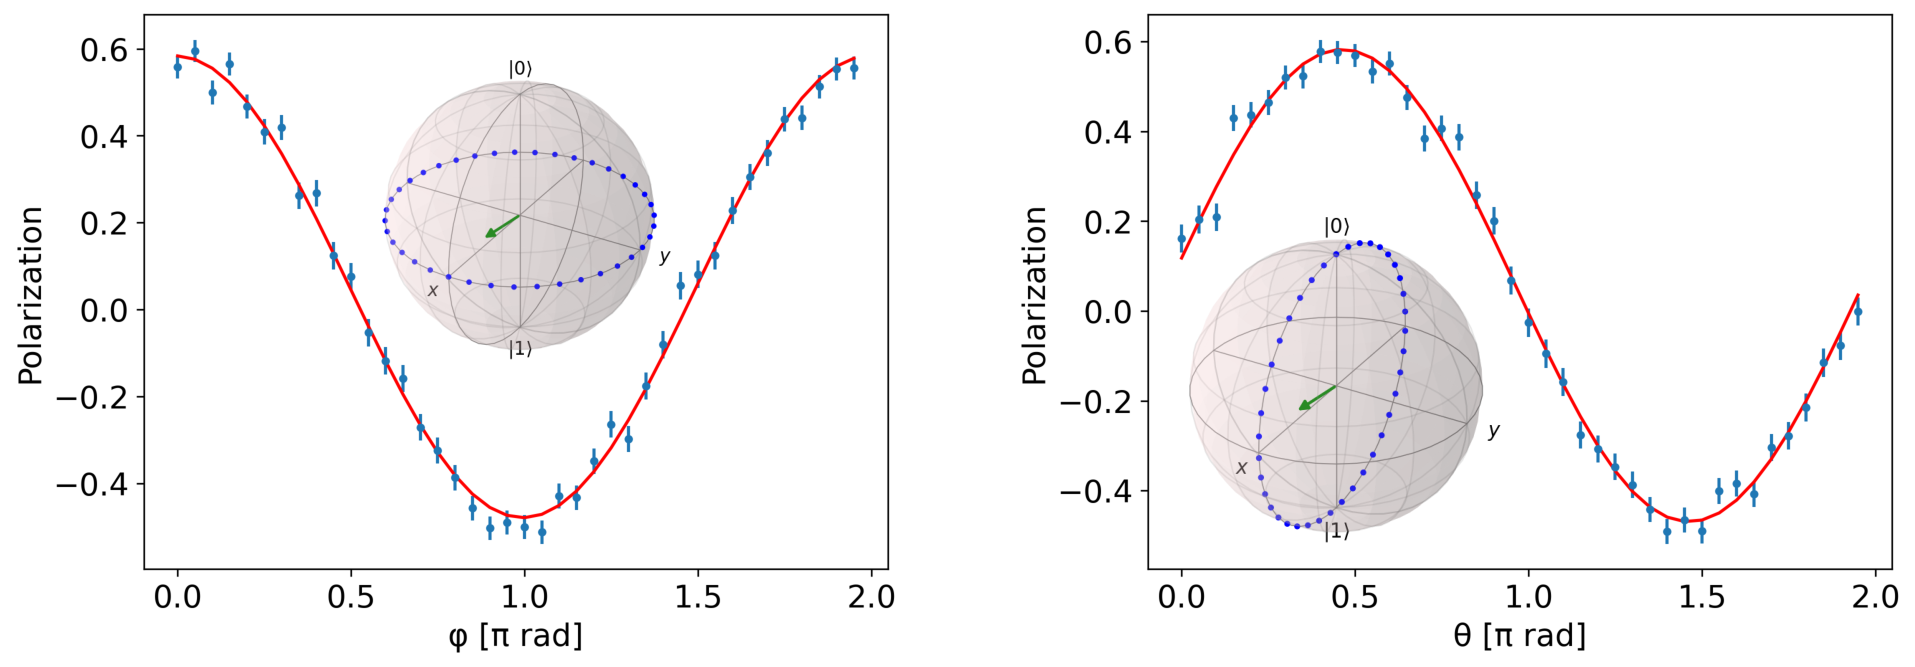
\includegraphics[width=0.85\linewidth]{Figures/flav_s_plus.pdf}
        \caption{The tomography of the control qubit's state after the interference protocol for measuring $S(\Psi_m, \Psi_m) = 1$. The measurement basis was scanned across two planes, see the Bloch sphere diagram (blue dotted circles), and the polarization $P$ was estimated from these measurements, fitting the Eq. \ref{eqn:estim} we have extracted the Bloch vector (orange arrow), from which we have made the estimate: $\tilde{S}(\Psi_m, \Psi_m) = 0.9$. Here the second ribbon's flavour was conditioned, Figure \ref{fig:cond_flav}.}
        \label{fig:flav_cond_res_plus}
    \end{subfigure}
        \begin{subfigure}{\textwidth}
        \centering
        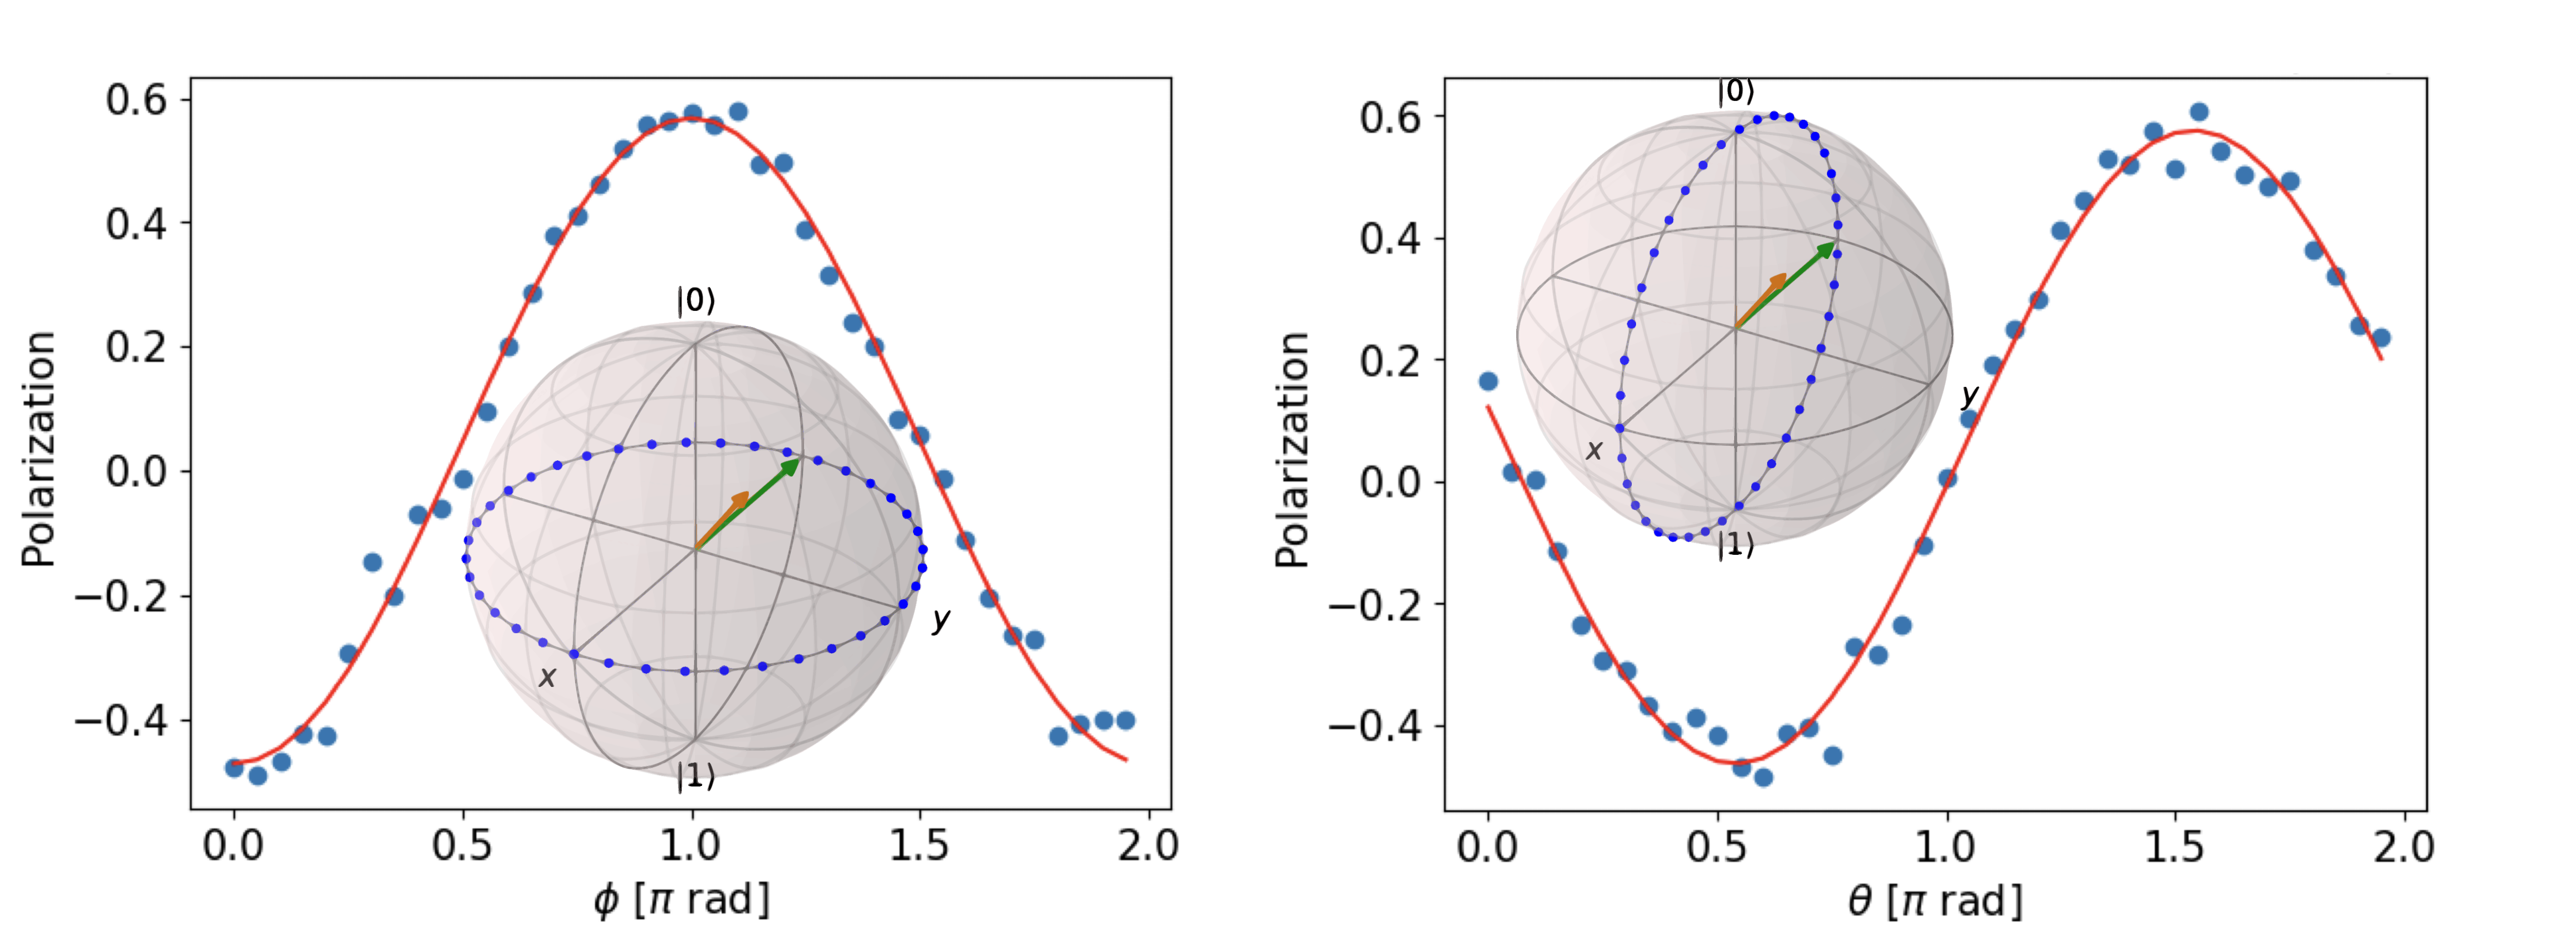
\includegraphics[width=0.8\linewidth]{Figures/flav_s_minus.pdf}
        \caption{The tomography of the control qubit's state after the interference protocol for measuring $S(\Psi_m, \tilde{\Psi}_m) = -1$. The measurement basis was scanned across two planes, see the Bloch sphere diagram (blue dotted circles), and the polarization $P$ was estimated from these measurements, fitting the Eq. \ref{eqn:estim} we have extracted the Bloch vector (orange arrow), from which we have made the estimate: $\tilde{S}(\Psi_m, \tilde{\Psi}_m) = -0.9$. Here the second ribbon's flavour was conditioned, Figure \ref{fig:cond_flav}.}
        \label{fig:flav_cond_res_minus}
    \end{subfigure}
    \begin{subfigure}{\textwidth}
        \centering
        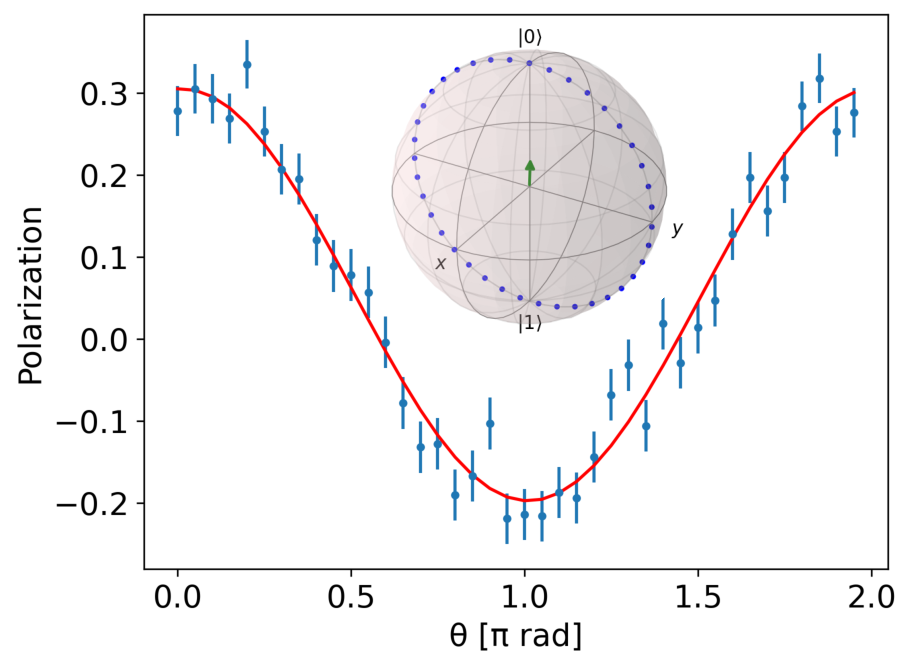
\includegraphics[width=0.4\linewidth]{Figures/flav_s_zero.pdf}
        \caption{The tomography of the control qubit's state after the interference protocol for measuring $S(\Psi_m, \Psi_r) = 0$. The measurement basis was scanned across two planes, see the Bloch sphere diagram (blue dotted circles), and the polarization $P$ was estimated from these measurements, fitting the Eq. \ref{eqn:estim} we have extracted the Bloch vector (orange arrow), from which we have made the estimate: $\tilde{S}(\Psi_m, \Psi_r) = 0$. Here the second ribbon's flavour was conditioned, Figure \ref{fig:cond_flav}.}
        \label{fig:flav_cond_res_zero}
    \end{subfigure}
    \caption{Numerical simulation of the S-matrix interference protocol and control qubit tomography.}
    \label{fig:flav_cond_res}
\end{figure*}

\begin{figure*}
        \centering
        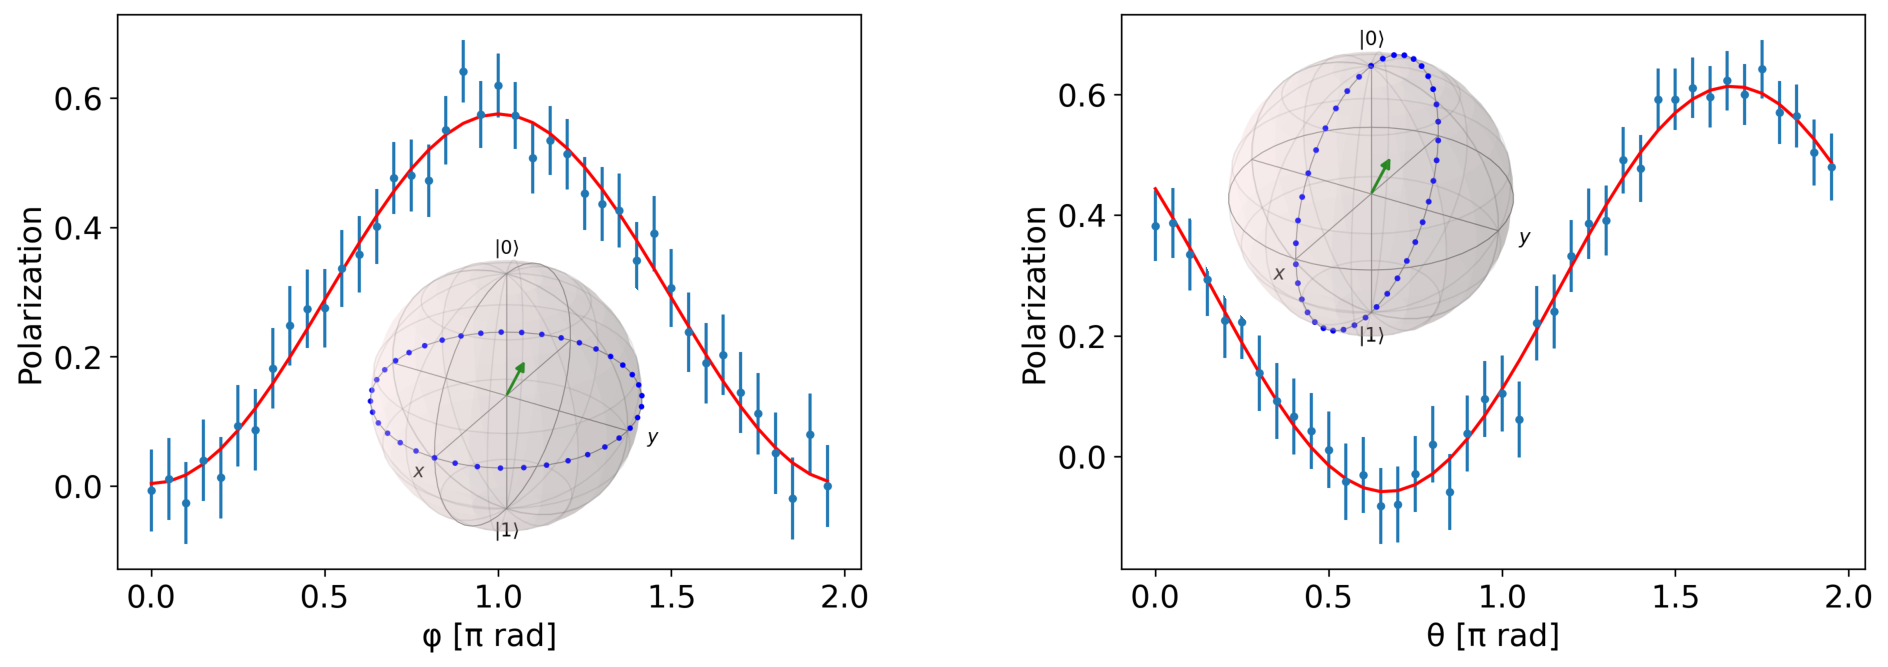
\includegraphics[width=\textwidth]{Figures/exist_s_minus.pdf}
        \caption{Numerical simulation of the S-matrix interference protocol and control qubit tomography: The tomography of the control qubit's state after the interference protocol for measuring $S(\Psi_m, \tilde{\Psi}_m) = -1$. The measurement basis was scanned across two planes, see the Bloch sphere diagram (blue dotted circles), and the polarization $P$ was estimated from these measurements, fitting the Eq. \ref{eqn:estim} we have extracted the Bloch vector (orange arrow), from which we have made the estimate: $\tilde{S}(\Psi_m, \tilde{\Psi}_m) = -0.6$. Here the second ribbon was fully conditioned, Figure \ref{fig:cond_ex}.}
        \label{fig:ex_cond_res}
\end{figure*}

\begin{figure*}
    \centering
    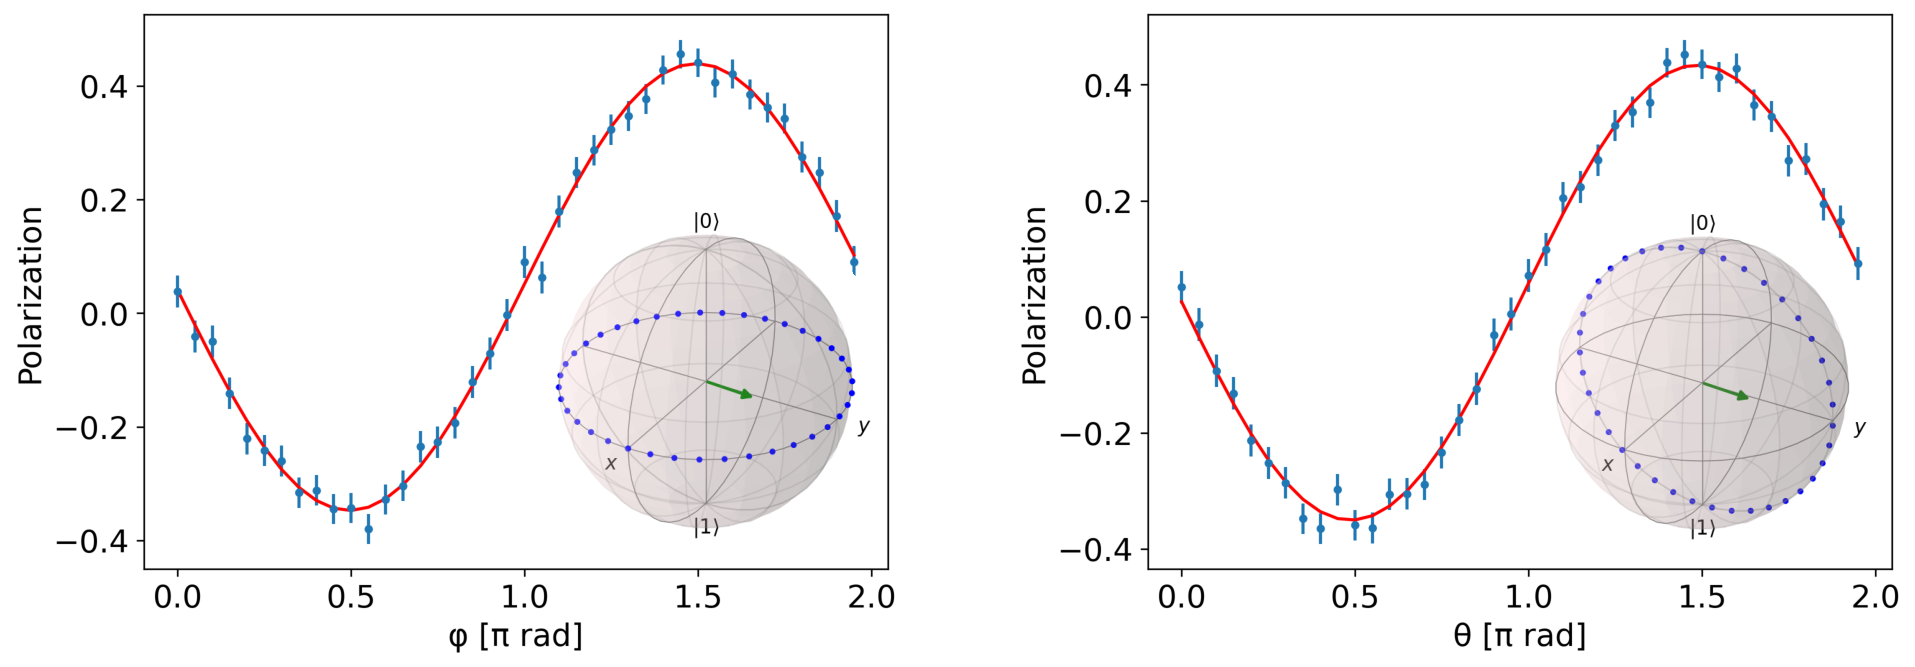
\includegraphics[width=\textwidth]{Figures/t_j_minus.pdf}
    \caption{Numerical simulation of the T-matrix interference protocol and control qubit tomography: The tomography of the control qubit's state after the interference protocol for measuring $T(\tilde{\Phi}_r, \tilde{\Phi}_r) = -i$. The measurement basis was scanned across two planes, see the Bloch sphere diagram (blue dotted circles), and the polarization $P$ was estimated from these measurements, fitting the Eq. \ref{eqn:estim} we have extracted the Bloch vector (orange arrow), from which we have made the estimate: $T(\tilde{\Phi}_r, \tilde{\Phi}_r) = -i$. Here the ribbon's path was conditioned, Figure \ref{fig:Tmat}.}
    \label{fig:t_mat_results}
\end{figure*}

In Figure \ref{fig:s_mat_res} we have a numerical result of our simulation of the S-matrix interference protocols. We have limited ourselves to a demonstrative selection of cases. Figure \ref{fig:ex_cond_res} shows the results of the protocol in which the existence of the second ribbon is conditioned on the state of the bit, Figure \ref{fig:cond_ex}. The systematic drift of the Bloch vector due to the effects of noise and readout bias are responsible for the underestimate of magnitude of the $\tilde{S}(\Psi_m, \tilde{\Psi}_m)$. Remember that the magnitude of the S-matrix element is dictated by the angle that the Bloch vector makes with respect to the z-axis, not the magnitude of the vector itself that is determined by the effective noise and readout.

The systematic drift is significantly less dramatic in the case of flavour conditioning protocol, Figure \ref{fig:flav_cond_res} for the results and Figure \ref{fig:cond_flav} for the protocol. Hence, the estimate of the magnitude of the S-matrix element, $\tilde{S}(\Psi_m, \tilde{\Psi}_m)$, is much closer to the theoretical value. This is due to the fact that the circuit implementing this protocol is much more shallow due to simpler forms of the conditional ribbon operators, one less Toffoli gate in the conditional multiplication circuit, Figure \ref{fig:flavCond}.

Furthermore, the T-matrix is remarkably well estimated by the path conditioning protocol, Figure \ref{fig:t_mat_results} for the results and Figure \ref{fig:Tmat} for the protocol.

The phases of all values are also estimated remarkably well.

\subsubsection{Circuit Depth}

In this section, we report the characteristics of the circuit implementing our interference protocols.

\jovan{ToDo.}

\section{Other Gauge Groups}

The anyons in the $D_4$ lattice gauge theory are not universal. 
When looking at compiled circuits for our experiments, they are Clifford or close to Clifford circuits.
They are efficiently classically simulatable, given we keep the number of Toffoli gates low.
The image of the braid group onto the transformations of the wavefunction as we braid anyons is finite, hence highly non-universal \cite{}.
This is all due to the simple structure of $D_4$, all of its subgroups are Abelian and the group is solvable.
However, if the gauge group in question is $S_3$ for example and if we allow measurements, we achieve computational universality.

In this section, we will discuss what carries over from our study further onto the case of the general group $G$ and in particular $S_3$

\jovan{ToDo.}



\section{Conclusions and Outlook}

\jovan{Start after the main text.}

\appendix

\section{Ribbon Types}\label{app:ribs}
\jovan{ToDo, a lot ToDo.}
\section{Representation Theory of $D_4$ and $D(D_4)$}\label{app:reps}
\jovan{$\ldots$}
\section{Circuits for $D_4$-related operations}\label{app:cirqs}
\section{Abelian anyons of $D_4$ gauge theory}\label{app:abl}
\section{Postsellection and one-qubit marginals}\label{app:marg}

\bibliographystyle{plain}
\bibliography{bibliography}


\end{document}
